% 本文件必须使用 XeLaTeX 编译（ctexart 不支持 pdfLaTeX）。
% 在 \documentclass 之前提前加载 fontspec，并静音其对 ctex 默认 Fandol 字体的
%   "Font ... does not contain requested Script CJK"
% 提示：这纯属字体元数据提示，不影响任何字符显示、换行与版面，
% 静音后编辑器 Problems 面板可完全干净；其他任何警告与错误仍照常报告。
\RequirePackage{fontspec}
\ExplSyntaxOn
\msg_redirect_name:nnn { fontspec } { no-script } { none }
\ExplSyntaxOff
\documentclass[UTF8,10pt,a4paper,twocolumn]{ctexart}

\usepackage[margin=1.8cm]{geometry}
\usepackage{amsmath,amssymb}
\usepackage{graphicx}
\usepackage{booktabs}
\usepackage{multirow}
\usepackage{url}
\usepackage[hidelinks]{hyperref}
\usepackage{cite}
\usepackage{caption}
\usepackage{subcaption}
\usepackage[table]{xcolor}
\usepackage{float}
\usepackage{cuted}
\usepackage{placeins}
\setlength{\dblfloatsep}{8pt plus 2pt minus 2pt}
\setlength{\textfloatsep}{8pt plus 2pt minus 2pt}
\setlength{\floatsep}{6pt plus 2pt minus 2pt}
\setlength{\intextsep}{6pt plus 2pt minus 2pt}

% 通栏（双栏浮动体）每页最多一个，避免宽表堆叠导致栏高计算错误与页脚重叠
\setcounter{dbltopnumber}{1}
\setcounter{topnumber}{2}
\setcounter{totalnumber}{3}
\usepackage{tikz}
\usetikzlibrary{arrows.meta,positioning,shapes.geometric,fit,calc}

\definecolor{pvoBlue}{HTML}{2F6FED}
\definecolor{pvoCyan}{HTML}{10B7B4}
\definecolor{pvoGreen}{HTML}{2AA876}
\definecolor{pvoOrange}{HTML}{F59E0B}
\definecolor{pvoRed}{HTML}{E05252}
\definecolor{pvoPurple}{HTML}{7C3AED}
\definecolor{pvoGray}{HTML}{F3F5F7}
\tikzset{
    pvoBlock/.style={rounded corners=2pt, draw=#1!75!black, fill=#1!14, very thick, align=center, inner sep=5pt, font=\scriptsize
},
    pvoSmall/.style={rounded corners=2pt, draw=#1!75!black, fill=#1!12, thick, align=center, inner sep=4pt, font=\scriptsize
},
    pvoArrow/.style={-{Latex[length=2.2mm]}, very thick, draw=black!65},
    pvoDashed/.style={-{Latex[length=2.0mm]}, thick, dashed, draw=black!45},
    pvoCurve/.style={very thick, draw=#1},
    pvoRisk/.style={fill=#1!16, draw=#1!75!black, very thick}
}

\title{\textbf{AVO：面向多模态移动机器人(4WIS)的概率速度障碍安全导航框架}}
\author{万宇轩\\
北京理工大学\\
\texttt{email@example.com}}
\date{}

\begin{document}
\maketitle

\begin{abstract}
动态环境中的局部导航要求机器人在有限观测、有限反应时间和不确定运动状态下判断候选动作的未来碰撞风险。在高频采样、低系统时延且障碍物状态充分可观测时，短时匀速外推通常是合理的局部近似；问题并不在于 VO 必然失效，而在于当前可用状态是否足以覆盖动作从观测到真正产生运动效果之间的有效反应窗口。本文据此将 AVO（Augur obstacles velocity）表述为部分可观测条件下的动作未来风险推理问题：给定观测历史、候选动作和有效反应窗口，估计该动作在短时预测窗内的碰撞概率，而不是简单复现当前帧的速度锥。面向四轮独立转向（4WIS）机器人的多模态速度空间，本文构建由动作映射、风险评估和安全过滤组成的导航框架，并以雷达方向间隙和短时车体包络推演形成动作条件风险估计；进一步引入局部观测不确定性，分析保守风险估计的作用。四种对比方法均运行在同一 4WIS 平台上，依次对应确定性 DRL-VO、单帧恒速 PVO、动作条件 AVO 及其不确定性感知扩展。基础动态障碍仿真中，10 个随机种子、每种方法 200 个 episode 的结果显示，动作条件风险过滤将成功率由 $64.0\%$ 提升至 $76.0\%$，碰撞率由 $30.0\%$ 降至 $10.0\%$；加入不确定性惩罚后碰撞率进一步降至 $4.0\%$，但超时率明显增加。为检验该结论的适用条件，本文进一步开展控制频率、有效时延、障碍物运动模式和历史状态四组受控实验，表 6--表 9 汇报相应的实际运行结果。
\end{abstract}

\textbf{关键词：}概率速度障碍；部分可观测导航；有效反应窗口；移动机器人导航；安全过滤；四轮独立转向；多模态运动；TD3

\section{引言}

移动机器人在仓储物流、工业巡检、灾害救援和特种作业等任务中需要在有限空间内持续感知环境、规避障碍物并到达目标点。传统差速或阿克曼底盘的运动自由度有限，在狭窄通道、泊车式转向、侧向避让和姿态受限通行等场景中容易受到转弯半径和非完整约束限制。四轮独立转向（4WIS）底盘通过独立控制各车轮转角，可实现阿克曼转向、横向转向和平行移动等多种运动模式，为复杂环境下的高机动导航提供了硬件基础。

已有 4WIS 规划研究表明，若将运动模式显式纳入状态或搜索空间，可以提升复杂环境中的路径质量和机动能力~\cite{bao2025hybrid}。但这类规划方法通常依赖较明确的地图、目标和障碍物模型；在动态障碍物、局部观测和传感器噪声条件下，局部策略还需要判断当前状态是否足以支持即将执行的动作。经典 VO 与动态窗口方法奠定了速度空间实时避障的几何基础~\cite{fiorini1998vo,fox1997dwa}，DRL-VO 则进一步将速度障碍特征与深度策略结合~\cite{xie2023drlvo}。需要强调的是，DRL-VO 已经使用短时 LiDAR 历史和邻近行人的运动学信息，因此本文并不把“使用历史”作为对所有 VO 方法的普遍纠正。更准确的问题是：在给定控制频率、系统时延和障碍物运动模式下，当前状态是否仍然是候选动作安全判断的充分状态。

本文将上述问题表述为状态充分性与有效反应窗口问题。设从传感器采样到机器人能够产生可观运动响应的时间为
\begin{equation}
    T_{\mathrm{eff}}=\Delta t_{\mathrm{sample}}+\Delta t_{\mathrm{infer}}+\Delta t_{\mathrm{comm}}+\Delta t_{\mathrm{act}}+T_{\mathrm{maneuver}}.
    \label{eq:effective_window}
\end{equation}
当 $T_{\mathrm{eff}}$ 很小、障碍物状态估计可靠且运动模式接近恒速时，当前帧 VO/PVO 可能已经足够；当 $T_{\mathrm{eff}}$ 与碰撞时间尺度同量级，或障碍物存在遮挡、转向和变速时，当前状态可能难以区分具有相同瞬时位置和速度但未来风险不同的运动过程。给定观测历史 $h_t$ 与候选动作 $a_t$，安全模块因此需要回答的是“该动作在有效反应窗口之后的未来窗口内发生碰撞的概率是多少”，而不是仅判断该动作是否落入当前帧速度锥。

本文选择 4WIS 机器人作为验证平台。其阿克曼、横向和平行移动模式显著扩展了可达速度集合，也使缺少风险约束的策略更容易产生高速近障动作。因而，4WIS 并非与 AVO 并列的独立创新，而是用于检验所提风险建模能否约束复杂动作空间的代表性载体。

本文的主要内容和贡献如下：
\begin{itemize}
    \item 将“历史信息是否必要”转化为可检验的状态充分性问题，明确区分高频低时延条件下当前帧 VO/PVO 的有效区域，以及部分可观测、有效反应窗口不可忽略时的潜在状态缺失。
    \item 提出适用于 4WIS 多模态速度空间的动作条件未来风险框架，以方向间隙和短时车体包络推演构造当前定量实验所用的解析近似，并在执行前过滤危险动作。
    \item 在统一的 4WIS 平台、观测条件和任务设置下比较 DRL-VO、普通 PVO、AVO 与 AVO-UQ；同时设计控制频率、有效时延、障碍物运动模式和历史状态条件的受控实验，用于界定方法收益的适用范围。
\end{itemize}

\section{相关工作}

\subsection{基于强化学习的机器人导航}

深度强化学习将机器人导航建模为序列决策问题，策略根据传感器观测直接输出控制动作。对于连续控制任务，DDPG、TD3 和 SAC 等 actor--critic 方法分别从确定性策略梯度、双 Q 网络与延迟更新、最大熵策略学习等角度改善连续动作优化~\cite{lillicrap2016ddpg,fujimoto2018td3,haarnoja2018sac}。在动态多智能体导航中，CADRL、去中心化多机器人避障和注意力式人群导航进一步说明，学习策略可以从局部观测中形成交互避让行为~\cite{chen2017cadrl,long2018decentralized,chen2019sarl,fan2020multirobot}。DRL-VO 在此基础上显式融合速度障碍特征，提高了动态人群场景中的几何可解释性~\cite{xie2023drlvo}。本文选用适合连续动作优化的 TD3 作为名义策略，并把研究重点放在独立于策略优化器的未来风险约束上。

\subsection{速度障碍与动态避障}

速度障碍方法通过分析机器人与障碍物在速度空间中的相对运动关系，判断某一速度在未来是否会导致碰撞。经典 VO 给出了单机器人相对速度碰撞锥~\cite{fiorini1998vo}，RVO 与 ORCA 通过互惠避让责任分配扩展到实时多智能体导航~\cite{vandenberg2008rvo,vandenberg2011orca}，GVO 则进一步处理更一般的机器人运动约束~\cite{wilkie2009gvo}。在预测窗口足够短、状态估计稳定且系统响应快速时，恒速外推是合理的一阶近似；其局限性取决于预测时域、障碍物运动变化以及从观测到动作生效的有效反应窗口，而不是由“匀速”二字本身决定。

为处理感知和运动不确定性，递归 PVO、PVO 与占据栅格融合以及概率互惠速度障碍分别从递归交互建模、空间占据概率和多机器人互惠约束角度扩展了速度障碍~\cite{kluge2006rpvo,fulgenzi2007pvo,gopalakrishnan2017prvo}。进一步的非参数 PVO 使用 Hilbert 空间嵌入表示难以预先指定分布形式的不确定性~\cite{poonganam2020pvo}。这些工作说明，概率化能够表达状态和观测噪声，但概率外壳并不自动解决隐状态、运动意图或动作执行时刻与预测起点不一致的问题。因此，普通 PVO 是本文重要的直接基线，而不是需要被否定的过时方法。

DRL-VO 将速度障碍特征嵌入学习策略，并结合短时 LiDAR 历史和周围行人运动学信息，在拥挤动态场景中学习目标趋近与避让行为~\cite{xie2023drlvo}。这一方向已经表明，历史信息在部分动态导航任务中具有实际价值；但其收益可能同时来自历史观测、显式运动学输入、策略表示能力和训练分布，不宜仅凭总体成功率归因于某一个因素。本文因此不声称当前帧 VO 在所有高频场景中失效，而是把频率、有效时延和障碍物运动模式作为受控变量，检验何时历史与动作条件风险带来可测增益。

在多机器人或多动态障碍物场景中，Social LSTM、Social GAN 与 Trajectron++ 等轨迹预测方法表明，动态主体的未来运动可能具有多模态、交互相关和动力学受限特征~\cite{alahi2016sociallstm,gupta2018socialgan,salzmann2020trajectron}。其中 Trajectron++ 还支持根据自车运动计划对其他主体进行条件预测，说明“历史 + 候选动作”本身并非孤立的新组件。本文关注的具体问题是：如何将这种状态充分性判断嵌入 4WIS 多模态候选动作的执行前安全过滤，并用受控实验报告其相对于当前帧确定性/概率 VO 的边界。由此，AVO 的核心主张应理解为一种面向有效反应窗口的动作风险建模框架，而不是对匀速近似的普遍否定。

\begin{figure*}[t]
    \centering

    \includegraphics[width=0.99\textwidth]{fig1_panels.pdf}
    % Former inline TikZ rendering of Fig. 1 (kept for traceability); it is
    % now replaced by the annotated figure supplied by the authors.
\iffalse
    \resizebox{0.99\textwidth}{!}{%
    \begin{tikzpicture}[
        font=\footnotesize,
        line join=round, line cap=round,
        panel/.style={rounded corners=3pt, draw=black!20, line width=0.55pt},
        badge/.style={fill=pvoBlue!82!black, rounded corners=1.6pt, inner sep=2.4pt,
                      text=white, font=\bfseries\small},
        ptitle/.style={anchor=west, font=\small, text=black!82},
        axis/.style={-{Latex[length=1.6mm]}, line width=0.7pt, draw=black!55},
        axislbl/.style={font=\scriptsize, text=black!60},
        riskone/.style={line width=1.1pt, draw=pvoRed!88!black},
        risktwo/.style={line width=1.1pt, draw=pvoBlue!82!black},
        meanline/.style={line width=0.62pt, densely dashed},
        candidate/.style={-{Latex[length=1.8mm]}, line width=1.3pt, draw=black!80},
        accepted/.style={-{Latex[length=1.8mm]}, line width=1.3pt, draw=pvoGreen!80!black},
        correction/.style={-{Latex[length=1.4mm]}, line width=0.7pt, densely dashed, draw=black!55},
        tag/.style={font=\scriptsize, fill=white, fill opacity=0.9, text opacity=1,
                    inner sep=1.3pt, rounded corners=1pt, text=black!80},
        obslbl/.style={font=\bfseries, text=black!80}
    ]

        % ================= (a) physical scene =================
        \begin{scope}
            \draw[panel] (-0.10,-0.12) rectangle (4.30,4.72);
            \node[badge] (ba) at (0.42,4.44) {(a)};
            \node[ptitle, right=6pt of ba] {双动态障碍场景};

            % bent future occupancy ribbons (start under the discs, which are drawn later)
            \draw[line width=0.44cm, draw=pvoRed!16, line cap=round]
                (3.20,3.30) .. controls (2.75,2.45) and (2.55,1.45) .. (2.45,0.75);
            \draw[line width=0.44cm, draw=pvoBlue!14, line cap=round]
                (3.70,2.05) .. controls (3.30,1.58) and (3.05,1.05) .. (2.95,0.55);
            \draw[densely dashed, line width=0.8pt, draw=pvoRed!70]
                (3.20,3.30) .. controls (2.75,2.45) and (2.55,1.45) .. (2.45,0.75);
            \draw[densely dashed, line width=0.8pt, draw=pvoBlue!70]
                (3.70,2.05) .. controls (3.30,1.58) and (3.05,1.05) .. (2.95,0.55);

            % robot with heading out of the nose
            \draw[rounded corners=2pt, fill=pvoBlue!16, draw=pvoBlue!85!black,
                  line width=0.95pt, rotate around={20:(1.05,1.15)}]
                (0.75,0.96) rectangle (1.35,1.34);
            \draw[-{Latex[length=1.6mm]}, line width=1.05pt, draw=pvoBlue!85!black]
                (1.33,1.25) -- (1.80,1.42) node[above right=-1pt, text=black!78]
                {$\mathbf v_r$};
            \node[anchor=north, font=\scriptsize, text=black!70] at (1.05,0.88) {4WIS};

            % obstacle o1
            \fill[pvoRed!17] (3.20,3.30) circle (0.42);
            \draw[riskone] (3.20,3.30) circle (0.42);
            \node[obslbl, text=pvoRed!88!black] at (3.20,3.30) {$o_1$};
            \draw[-{Latex[length=1.5mm]}, riskone] (3.00,2.93) -- (2.79,2.53);
            \node[obslbl, text=pvoRed!88!black, anchor=east] at (2.45,2.75)
                {$\hat{\mathbf v}_{o_1}$};

            % obstacle o2
            \fill[pvoBlue!15] (3.70,2.05) circle (0.44);
            \draw[risktwo] (3.70,2.05) circle (0.44);
            \node[obslbl, text=pvoBlue!88!black] at (3.70,2.05) {$o_2$};
            \draw[-{Latex[length=1.5mm]}, risktwo] (3.42,1.72) -- (3.13,1.38);
            \node[obslbl, text=pvoBlue!88!black, anchor=west] at (3.55,1.24)
                {$\hat{\mathbf v}_{o_2}$};

            % annotation + leader
            \node[anchor=north west, align=left, font=\scriptsize, text=black!68]
                at (0.22,4.16) {转向/变速导致\\未来占据区域弯曲};
            \draw[densely dotted, line width=0.6pt, draw=black!38, -{Latex[length=1.2mm]}]
                (2.20,3.38) .. controls (2.50,3.05) and (2.72,2.65) .. (2.80,2.40);
        \end{scope}

        % ================= (b) current-frame VO / PVO =================
        \begin{scope}[xshift=4.80cm]
            \draw[panel] (-0.10,-0.12) rectangle (4.30,4.72);
            \node[badge] (bb) at (0.42,4.44) {(b)};
            \node[ptitle, right=6pt of bb] {当前帧 VO / PVO};

            \begin{scope}[shift={(0.95,0.95)}, scale=0.85, shift={(-0.48,-0.52)}]
                \draw[axis] (0.48,0.52) -- (4.00,0.52)
                    node[below left=-1pt, axislbl] {$v_{\mathrm{rel},x}$};
                \draw[axis] (0.48,0.52) -- (0.48,3.82)
                    node[left, axislbl] {$v_{\mathrm{rel},y}$};
                \node[anchor=north east, font=\scriptsize, text=black!58]
                    at (0.48,0.52) {$\mathbf 0$};

                \path[fill=pvoRed!13]
                    (0.48,0.52) -- (3.82,3.86)
                    .. controls (4.01,3.37) and (3.98,2.93) .. (3.69,2.53) -- cycle;
                \draw[riskone] (0.48,0.52) -- (3.82,3.86);
                \draw[riskone] (0.48,0.52) -- (3.69,2.53);
                \draw[riskone] (3.82,3.86) .. controls (4.01,3.37) and (3.98,2.93) .. (3.69,2.53);
                \draw[meanline, pvoRed!64] (0.48,0.52) -- (3.82,3.16);
                \node[tag, text=pvoRed!88!black] at (3.28,3.22) {$\mathrm{VO}^{T}_{1}$};

                \path[fill=pvoBlue!11]
                    (0.48,0.52) -- (3.84,2.42)
                    .. controls (4.00,1.96) and (3.95,1.49) .. (3.76,1.08) -- cycle;
                \draw[risktwo] (0.48,0.52) -- (3.84,2.42);
                \draw[risktwo] (0.48,0.52) -- (3.76,1.08);
                \draw[risktwo] (3.84,2.42) .. controls (4.00,1.96) and (3.95,1.49) .. (3.76,1.08);
                \draw[meanline, pvoBlue!62] (0.48,0.52) -- (3.86,1.72);
                \node[tag, text=pvoBlue!88!black] at (3.36,1.50) {$\mathrm{VO}^{T}_{2}$};

                \draw[candidate] (0.48,0.52) -- (2.95,2.13)
                    node[pos=0.60, above left=1.5pt, tag, text=black!76] {$\mathbf v_t^{\mathrm{cand}}$};
                \draw[accepted] (0.48,0.52) -- (1.58,3.45)
                    node[pos=0.80, left, tag, text=pvoGreen!66!black] {$\mathbf v_t^{\mathrm{safe}}$};
                \draw[correction] (2.95,2.13) -- (1.58,3.45);
                \node[anchor=south east, font=\scriptsize, text=black!62] at (2.72,3.00)
                    {$\Delta\mathbf v_{\mathrm{safe}}$};
                \node[anchor=west, font=\scriptsize, text=black!58] at (0.64,0.02)
                    {$\mathrm{VO}^{T}=\mathrm{VO}^{T}_{1}\cup\mathrm{VO}^{T}_{2}$};
            \end{scope}
        \end{scope}

        % ================= (c) neural-pvo =================
        \begin{scope}[xshift=9.60cm]
            \draw[panel] (-0.10,-0.12) rectangle (4.30,4.72);
            \node[badge] (bc) at (0.42,4.44) {(c)};
            \node[ptitle, right=6pt of bc] {AVO（本文）};

            \begin{scope}[shift={(0.95,0.95)}, scale=0.85, shift={(-0.48,-0.52)}]
                \draw[axis] (0.48,0.52) -- (4.00,0.52)
                    node[below left=-1pt, axislbl] {$v_{\mathrm{rel},x}$};
                \draw[axis] (0.48,0.52) -- (0.48,3.82)
                    node[left, axislbl] {$v_{\mathrm{rel},y}$};
                \node[anchor=north east, font=\scriptsize, text=black!58]
                    at (0.48,0.52) {$\mathbf 0$};

                \path[fill=pvoRed!13]
                    (0.48,0.52)
                    .. controls (1.52,1.72) and (2.13,3.25) .. (3.90,3.88)
                    .. controls (3.95,3.33) and (3.88,2.88) .. (3.65,2.50)
                    .. controls (2.72,2.35) and (1.64,1.02) .. (0.48,0.52) -- cycle;
                \draw[riskone]
                    (0.48,0.52) .. controls (1.52,1.72) and (2.13,3.25) .. (3.90,3.88);
                \draw[riskone]
                    (0.48,0.52) .. controls (1.64,1.02) and (2.72,2.35) .. (3.65,2.50);
                \draw[riskone] (3.90,3.88) .. controls (3.95,3.33) and (3.88,2.88) .. (3.65,2.50);
                \draw[meanline, pvoRed!65]
                    (0.48,0.52) .. controls (1.72,1.35) and (2.38,2.73) .. (3.78,3.18);
                \draw[dotted, line width=0.75pt, pvoRed!62]
                    (1.25,1.29) .. controls (1.86,1.88) and (2.46,2.92) .. (3.64,3.34);
                \node[tag, text=pvoRed!88!black] at (3.32,3.18) {$\mathcal R_{1,\eta}$};

                \path[fill=pvoBlue!11]
                    (0.48,0.52)
                    .. controls (1.45,0.88) and (2.17,2.25) .. (3.86,2.52)
                    .. controls (4.00,2.06) and (3.96,1.52) .. (3.73,1.04)
                    .. controls (2.55,1.32) and (1.53,0.63) .. (0.48,0.52) -- cycle;
                \draw[risktwo]
                    (0.48,0.52) .. controls (1.45,0.88) and (2.17,2.25) .. (3.86,2.52);
                \draw[risktwo]
                    (0.48,0.52) .. controls (1.53,0.63) and (2.55,1.32) .. (3.73,1.04);
                \draw[risktwo] (3.86,2.52) .. controls (4.00,2.06) and (3.96,1.52) .. (3.73,1.04);
                \draw[meanline, pvoBlue!64]
                    (0.48,0.52) .. controls (1.55,0.77) and (2.30,1.78) .. (3.82,1.72);
                \draw[dotted, line width=0.75pt, pvoBlue!62]
                    (1.13,0.81) .. controls (1.79,1.04) and (2.48,1.85) .. (3.60,1.91);
                \node[tag, text=pvoBlue!88!black] at (3.30,1.58) {$\mathcal R_{2,\eta}$};

                \draw[candidate] (0.48,0.52) -- (3.02,2.08)
                    node[pos=0.60, above left=1.5pt, tag, text=black!76] {$\mathbf v_t^{\mathrm{cand}}$};
                \draw[accepted] (0.48,0.52) -- (1.52,3.54)
                    node[pos=0.80, left, tag, text=pvoGreen!66!black] {$\mathbf v_t^{\star}$};
                \draw[correction] (3.02,2.08) -- (1.52,3.54);
                \node[anchor=south east, font=\scriptsize, text=black!62] at (2.95,3.45)
                    {$\Delta\mathbf v_{\mathrm{AVO}}$};
                \node[anchor=west, font=\scriptsize, text=black!58] at (0.64,0.02)
                    {$\mathcal R_{\eta}=\mathcal R_{1,\eta}\cup\mathcal R_{2,\eta}$};
            \end{scope}
        \end{scope}

        % ================= shared legend =================
        \begin{scope}[yshift=-0.95cm]
            \fill[pvoRed!13] (0.95,-0.13) rectangle (1.29,0.13);
            \draw[riskone, line width=0.9pt] (0.95,-0.13) rectangle (1.29,0.13);
            \node[anchor=west, font=\footnotesize, text=black!80] at (1.43,0.00)
                {$o_1$ 危险集合};

            \fill[pvoBlue!11] (4.23,-0.13) rectangle (4.57,0.13);
            \draw[risktwo, line width=0.9pt] (4.23,-0.13) rectangle (4.57,0.13);
            \node[anchor=west, font=\footnotesize, text=black!80] at (4.71,0.00)
                {$o_2$ 危险集合};

            \draw[candidate] (7.51,0.00) -- (7.95,0.00);
            \node[anchor=west, font=\footnotesize, text=black!80] at (8.09,0.00)
                {策略候选速度};

            \draw[accepted] (11.07,0.00) -- (11.51,0.00);
            \node[anchor=west, font=\footnotesize, text=black!80] at (11.65,0.00)
                {过滤后速度};
        \end{scope}
    \end{tikzpicture}}
\fi
    \caption{双动态障碍场景下当前帧 VO/PVO 与动作条件 AVO 的对比。(a) 4WIS 同时遭遇障碍物 $o_1$ 和 $o_2$，二者在预测窗内存在转向或变速；(b) DRL-VO 依据当前速度估计构造直线边界的确定性危险集合，普通 PVO 则在相同的单帧恒速外推上引入状态与速度不确定性，将二值集合扩展为概率危险区域，但二者均以当前时刻作为预测起点；(c) AVO 根据历史观测 $h_t$、候选动作 $a$ 和全栈时延后的未来窗口分别估计 $\mathcal R_{i,\eta}=\{\mathbf v(a):p_{\psi}(\mathrm{coll}_i\mid h_t,a)\ge\eta,\ a\in\mathcal A\}$。为便于比较，(b) 和 (c) 均绘制在相对速度空间，并以原点作为共同速度参考。半透明区域为高风险速度集合，点状内曲线为等概率轮廓；障碍物的非线性运动和预测不确定性使 AVO 边界发生弯曲与扩张。候选速度落入任一风险集合时，安全过滤器选择并集之外的安全替代速度；$\Delta\mathbf v_{\mathrm{AVO}}=\mathbf v_t^{\star}-\mathbf v_t^{\mathrm{cand}}$ 表示该速度修正量，并非欧氏意义的最小速度偏移量。}
    \label{fig:curved_pvo_cone}
\end{figure*}

\subsection{4WIS 多模态运动规划}

4WIS 底盘的关键优势在于运动模式丰富。阿克曼模式适合常规前向行驶和平滑转弯，横向模式适合狭窄空间中的侧向位移，平行移动模式则允许机器人在保持车体姿态不变的情况下沿任意方向平移。Bao 等提出的多模态 Hybrid A* 将运动模式作为状态维度，并通过模式切换代价、多模态曲线和终端连接策略提升 4WIS 规划效果~\cite{bao2025hybrid}。本文借鉴这一思路，但研究对象从全局搜索规划转向局部动态导航：强化学习策略不直接搜索 $(x,y,\theta,m)$ 图，而是在每个控制周期根据雷达观测和目标相对位姿选择 4WIS 运动模式，并由 AVO 模块评估候选动作的碰撞风险。

\subsection{不确定性估计与安全强化学习}

安全强化学习通常通过约束策略优化、动作投影或外部安全层限制训练和执行阶段的危险探索~\cite{garcia2015safe,achiam2017cpo,dalal2018safetylayer}；控制障碍函数则提供了将名义动作投影到安全可行集的解析工具~\cite{ames2017cbf}。本文同样采用“策略提出候选动作、风险模块负责执行前过滤”的分层结构，但安全判据由面向未来窗口的 AVO 风险给出，以适配动态障碍物和 4WIS 多模态速度空间。

在动态场景中，碰撞概率预测模型还可能遇到训练分布之外的障碍物运动模式。若只输出单一概率，策略难以区分“低风险”与“模型不确定但表面低风险”的动作。MC Dropout、深度集成分别提供了近似贝叶斯和多模型集成的不确定性估计方式~\cite{gal2016dropout,lakshminarayanan2017ensembles}，而认知不确定性与数据不确定性的区分有助于明确保守惩罚的来源~\cite{kendall2017uncertainties}。本文以候选方向附近的局部间隙构造可控的不确定性近似，并通过独立消融分析保守风险修正对碰撞与超时的影响。

\section{问题定义与总体框架}

本文考虑局部观测下的动态导航问题。策略分支根据目标相对状态、上一时刻车体速度和当前运动模式生成候选动作 $a_t=[u_t,\xi_t,q_t]$；风险分支可进一步维护最近 $K$ 帧二维激光雷达，以估计候选动作在有效反应窗口后的未来碰撞风险，并由动作映射层得到车体速度 $[v_x,v_y,\omega]$。如图~\ref{fig:pipeline} 所示，策略分支负责目标导向的动作生成，风险分支负责候选动作的风险评估与不确定性估计，安全层仅允许满足风险约束的动作进入执行环节。该分解将任务性能优化与执行安全判别解耦，使同一风险约束能够作用于不同 4WIS 运动模式。

\begin{figure*}[t]
    \centering

    \includegraphics[width=0.99\textwidth]{fig2_pipeline.pdf}
    \caption{AVO 的训练与安全执行框架。黑色箭头表示观测编码及融合特征的前向传递；青色箭头表示 Critic 对 Actor 的策略更新；橙色箭头表示候选动作的风险估计、安全过滤、4WIS 模式映射及环境执行；绿色箭头表示 IRSim 生成的奖励与状态转移对 Critic 的反馈更新。安全车体速度同时送入 IRSim 训练环境与 Gazebo 高保真验证环境。}
    \label{fig:pipeline}
\end{figure*}

% Retain the former inline TikZ implementation for traceability.
\iffalse

\begin{figure*}[t]
    \centering

    \resizebox{0.99\textwidth}{!}{
    \begin{tikzpicture}[
        font=\scriptsize
,
        net/.style={circle, draw=black!58, line width=0.55pt, fill=white,
                    minimum size=3.1mm, inner sep=0pt},
        netActor/.style={net, fill=pvoOrange!18, draw=pvoOrange!80!black},
        netCritic/.style={net, fill=pvoBlue!16, draw=pvoBlue!78!black},
        netRisk/.style={net, fill=pvoRed!15, draw=pvoRed!80!black},
        frame/.style={rounded corners=2pt, draw=black!28, line width=0.55pt, fill=white},
        thinlink/.style={line width=0.35pt, draw=black!42},
        flow/.style={-{Latex[length=1.8mm]}, line width=1.0pt, draw=black!67},
        trainflow/.style={-{Latex[length=1.7mm]}, line width=0.9pt, draw=pvoBlue!75!black},
        deployflow/.style={-{Latex[length=1.7mm]}, line width=0.9pt, draw=pvoRed!78!black}
    ]
        % Multi-source observation.
        \node[font=\bfseries] at (0.92,6.08) {多源观测};
        \draw[frame, fill=pvoBlue!4] (-0.10,2.90) rectangle (1.94,5.88);
        \foreach \dx/\dy in {0.00/0.00,0.10/0.10,0.20/0.20}{
            \draw[fill=white, draw=pvoBlue!55, line width=0.45pt]
                (0.25+\dx,4.63+\dy) rectangle (1.43+\dx,5.43+\dy);
            \draw[pvoBlue!48, line width=0.38pt] (0.84+\dx,5.03+\dy) -- (0.38+\dx,5.26+\dy);
            \draw[pvoBlue!48, line width=0.38pt] (0.84+\dx,5.03+\dy) -- (1.31+\dx,5.32+\dy);
            \draw[pvoBlue!48, line width=0.38pt] (0.84+\dx,5.03+\dy) -- (1.23+\dx,4.74+\dy);
        }
        \node[align=center, font=\tiny] at (0.95,4.36)
            {多帧 LiDAR 序列};
        \node[pvoSmall=pvoCyan, minimum width=1.70cm, minimum height=0.62cm]
            (robotstate) at (0.92,3.35) {目标、速度与模式\\$[g_t,\mathbf v_t,e(m_t)]$};

        % Branch encoders inspired by NavRL.
        \node[font=\bfseries] at (3.02,6.08) {分支特征提取};
        \node[frame, fill=pvoBlue!5, minimum width=1.66cm, minimum height=1.26cm]
            (temporal) at (3.02,4.95) {};
        \foreach \x in {2.56,2.75,2.94}{
            \draw[fill=pvoBlue!13, draw=pvoBlue!68!black, line width=0.55pt]
                (\x,4.66) -- ++(0.30,0.13) -- ++(0,0.60) -- ++(-0.30,-0.13) -- cycle;
        }
        \node[align=center, font=\tiny] at (3.02,4.22)
            {LiDAR MLP--GRU};
        \node[frame, fill=pvoCyan!5, minimum width=1.66cm, minimum height=1.16cm]
            (stateenc) at (3.02,3.30) {};
        \foreach \x in {2.60,2.82,3.04}{
            \draw[fill=pvoCyan!13, draw=pvoCyan!68!black, line width=0.55pt]
                (\x,3.04) rectangle ++(0.16,0.62);
        }
        \node[align=center, text width=1.45cm] at (3.02,2.67)
            {状态 MLP\\特征编码器};
        \draw[flow] (1.76,5.05) -- (temporal.west);
        \draw[flow] (robotstate.east) -- (stateenc.west);

        % Fused latent representation.
        \draw[rounded corners=1pt, fill=pvoCyan!24, draw=pvoCyan!75!black,
              line width=0.75pt] (4.26,2.12) rectangle (4.48,5.64);
        \node[rotate=90, font=\bfseries, text=pvoCyan!55!black] at (4.37,3.88)
            {融合嵌入 $e_t$};
        \draw[flow] (temporal.east) -- (4.26,4.95);
        \draw[flow] (stateenc.east) -- (4.26,3.30);

        % Actor neural network.
        \node[font=\bfseries, text=pvoOrange!75!black] at (5.40,5.82)
            {Actor 策略};
        \foreach \y [count=\i] in {5.33,4.96,4.59}
            \node[netActor] (a1-\i) at (5.05,\y) {};
        \foreach \y [count=\j] in {5.43,5.10,4.77,4.44}
            \node[netActor] (a2-\j) at (5.68,\y) {};
        \foreach \y [count=\k] in {5.30,4.94,4.58}
            \node[netActor] (a3-\k) at (6.32,\y) {};
        \foreach \i in {1,...,3} \foreach \j in {1,...,4}
            \draw[thinlink] (a1-\i) -- (a2-\j);
        \foreach \j in {1,...,4} \foreach \k in {1,...,3}
            \draw[thinlink] (a2-\j) -- (a3-\k);
        \node[align=center, text=black!67] at (6.35,4.18)
            {$a_t=[u_t,\xi_t,q_t]$};
        \draw[flow] (4.48,4.96) -- (a1-2);

        % Critic neural network.
        \node[font=\bfseries, text=pvoBlue!75!black] at (5.45,3.45)
            {TD3 Critic};
        \foreach \y [count=\i] in {2.98,2.66,2.34,2.02}
            \node[netCritic] (c1-\i) at (5.05,\y) {};
        \foreach \y [count=\j] in {3.02,2.70,2.38,2.06}
            \node[netCritic] (c2-\j) at (5.68,\y) {};
        \foreach \y [count=\k] in {2.84,2.52,2.20}
            \node[netCritic] (c3-\k) at (6.32,\y) {};
        \foreach \i in {1,...,4} \foreach \j in {1,...,4}
            \draw[thinlink] (c1-\i) -- (c2-\j);
        \foreach \j in {1,...,4} \foreach \k in {1,...,3}
            \draw[thinlink] (c2-\j) -- (c3-\k);
        \node[text=black!67] at (6.34,1.78) {$Q_1,Q_2$};
        \draw[flow] (4.48,2.34) -- (c1-3);

        % AVO risk head conditioned on history and action.
        \node[font=\bfseries, text=pvoRed!78!black] at (7.98,5.82)
            {AVO};
        \foreach \y [count=\i] in {5.55,4.94,4.50}
            \node[netRisk] (r1-\i) at (7.15,\y) {};
        \foreach \y [count=\j] in {5.34,5.02,4.70,4.38}
            \node[netRisk] (r2-\j) at (7.72,\y) {};
        \foreach \y [count=\k] in {5.14,4.70}
            \node[netRisk] (r3-\k) at (8.30,\y) {};
        \foreach \i in {1,...,3} \foreach \j in {1,...,4}
            \draw[thinlink] (r1-\i) -- (r2-\j);
        \foreach \j in {1,...,4} \foreach \k in {1,...,2}
            \draw[thinlink] (r2-\j) -- (r3-\k);
        \node[align=center, text=pvoRed!75!black] at (8.28,4.24)
            {$\hat p_{\mathrm{coll}},\,\hat\sigma_p$};
        \draw[deployflow] (a3-2) -- (r1-2);
        \draw[deployflow] (4.48,5.55) -- (r1-1);

        % Deployment safety path.
        \node[pvoBlock=pvoRed, minimum width=1.65cm, minimum height=0.78cm]
            (filter) at (9.50,4.92) {风险约束\\安全过滤};
        \node[pvoBlock=pvoPurple, minimum width=1.72cm, minimum height=0.78cm]
            (mapper) at (11.36,4.92) {4WIS 动作\\模式映射};
        \node[pvoBlock=pvoGreen, minimum width=1.70cm, minimum height=0.78cm]
            (command) at (13.25,4.92) {安全车体速度\\$[v_x,v_y,\omega]$};
        \coordinate (riskout) at (8.55,4.92);
        \draw[thinlink] (r3-1.east) -- (riskout);
        \draw[thinlink] (r3-2.east) -- (riskout);
        \draw[deployflow] (riskout) -- (filter.west);
        \draw[deployflow] (filter) -- (mapper);
        \draw[deployflow] (mapper) -- (command);
        \node[pvoSmall=pvoGray, minimum width=2.20cm, minimum height=0.48cm,
              font=\tiny] (proxy) at (9.50,3.72)
            {当前实现：间隙 + rollout + UQ 几何代理};
        \draw[densely dashed, line width=0.75pt, draw=black!42]
            (proxy.north) -- (filter.south);
        \node[font=\bfseries, text=pvoRed!75!black] at (11.42,5.88)
            {部署与安全执行};

        % Training and high-fidelity scene thumbnails.
        \node[font=\bfseries, text=pvoBlue!75!black] at (8.45,3.38)
            {IRSim 并行训练};
        \node[draw=pvoBlue!65!black, line width=0.75pt, inner sep=1.5pt,
              label={[font=\tiny,text=black!62]below:动态障碍训练场景}]
            (irsim) at (8.45,2.20)
            {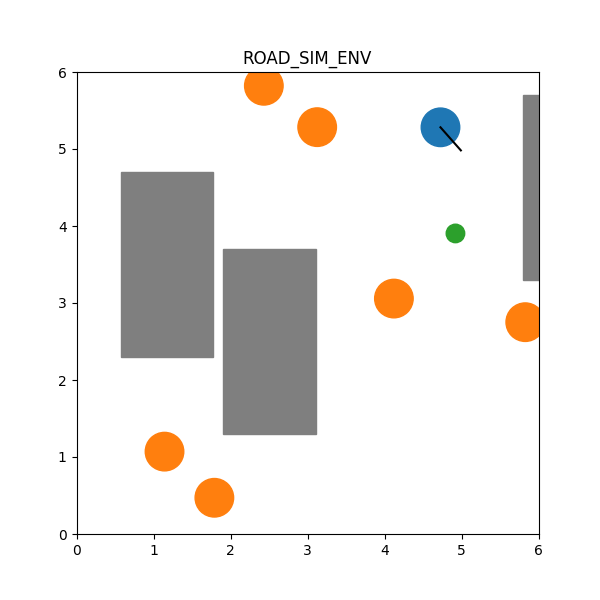
\includegraphics[width=2.15cm,height=1.62cm]{../images/irsim_frame.png}};
        \node[pvoSmall=pvoOrange, minimum width=1.55cm, minimum height=0.55cm]
            (reward) at (10.55,2.20) {奖励与转移\\$(r_t,s_{t+1})$};
        \node[font=\bfseries, text=pvoGreen!68!black] at (15.65,5.88)
            {Gazebo 高保真验证};
        \node[draw=pvoGreen!65!black, line width=0.75pt, inner sep=1.5pt,
              label={[font=\tiny,text=black!62]below:4WIS 与动态障碍场景}]
            (gazebo) at (15.65,4.92)
            {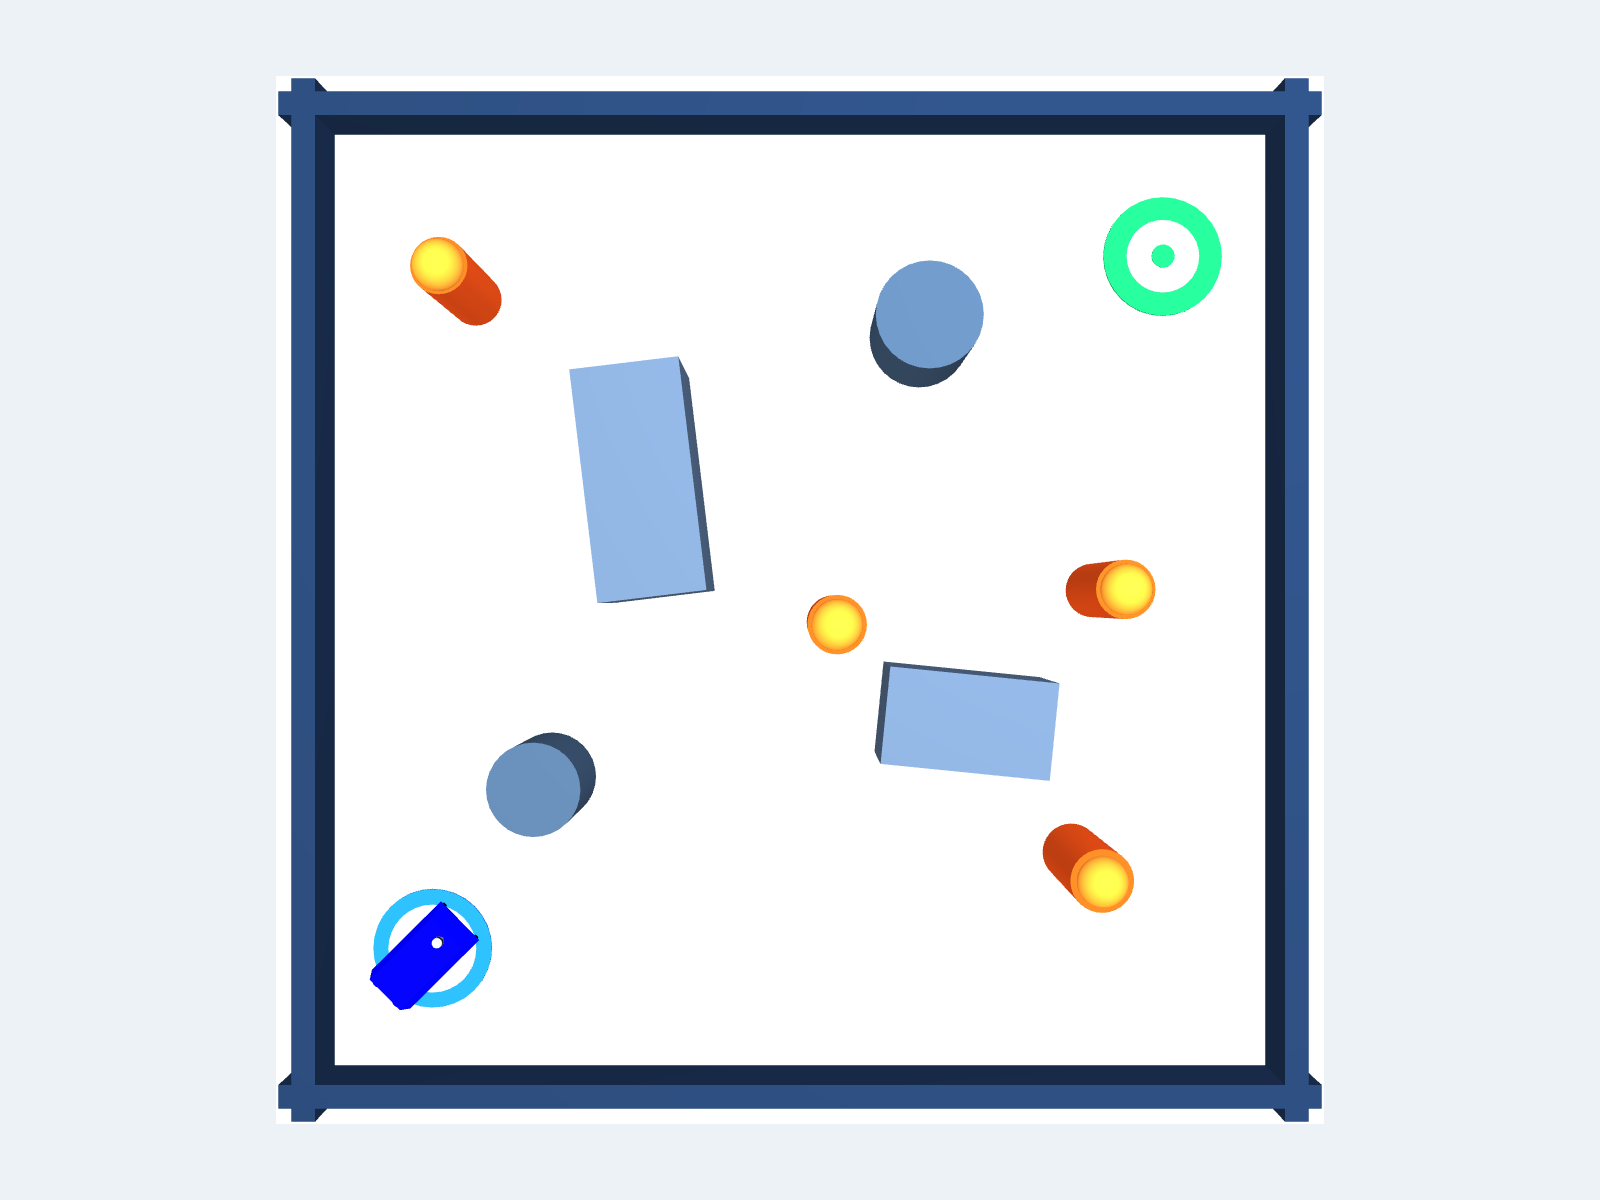
\includegraphics[width=2.35cm,height=1.62cm]{../images/gazebo_neural_pvo_overview.png}};
        \draw[trainflow] (c3-3.east) -- (irsim.west);
        \draw[trainflow] (irsim.east) -- (reward.west);
        \draw[pvoDashed] (command.east) -- (gazebo.west);
        \draw[-{Latex[length=1.7mm]}, line width=0.9pt, draw=pvoBlue!75!black]
            (10.55,0.72) -- (4.70,0.72);
        \node[font=\tiny, text=pvoBlue!65!black] at (7.63,0.96)
            {经验回放与 Actor--Critic 参数更新};
    \end{tikzpicture}}
    \caption{AVO 的训练与安全执行框架。多帧 LiDAR 序列和机器人内部状态由独立编码器提取特征，融合嵌入同时输入 TD3 Actor--Critic 和动作条件 AVO 风险头。Actor 产生 4WIS 紧凑动作，风险头预测候选动作的碰撞概率与不确定性，安全过滤后经运动模式映射得到车体速度。IRSim 构成强化学习训练闭环，Gazebo 提供含真实 4WIS 模型的高保真验证接口。虚线几何代理模块对应本文当前实验实现；完整 MLP--GRU 风险头是后续利用 4WIS 时序数据训练的目标模型。}
    \label{fig:pipeline_legacy}
\end{figure*}
\fi

\subsection{局部导航任务}

环境在每个离散控制时刻返回激光雷达扫描、目标相对距离与方向、机器人运动状态以及终止信号。本文所有对比方法均以 4WIS 为统一验证平台，其瞬时运动表示为车体系速度 $\mathbf v_b=[v_x,v_y,\omega]$，并通过阿克曼、横向与平行移动模式生成不同的可行速度。碰撞检测采用姿态相关的矩形车体包络。一次 episode 在到达目标、发生碰撞或达到时间上限时终止。该任务同时包含目标趋近、静态几何约束和动态交互风险，因而要求策略在通行效率与安全裕度之间进行权衡。4WIS 在本文中仅作为具有复杂可达速度集合的理论验证平台，实验不讨论其相对于其他底盘形式的性能优势。

\subsection{观测空间与动作空间}

四种方法共享 53 维 4WIS 观测，包括 42 维降采样雷达、3 维目标相对信息、3 维上一时刻车体系速度 $\mathbf v_{b,t-1}=[v_{x,t-1},v_{y,t-1},\omega_{t-1}]$、2 维目标朝向误差表示和 3 维当前运动模式 one-hot 编码：
\begin{equation}
\begin{aligned}
    o_t=[&z_t,d_t,\cos\alpha_t,\sin\alpha_t,v_{x,t-1},v_{y,t-1},\omega_{t-1},\\
    &\cos\Delta\theta_t,\sin\Delta\theta_t,e(m_t)].
\end{aligned}
\end{equation}
统一的高层动作定义为
\begin{equation}
    a_t=[u_t,\xi_t,q_t], \quad u_t,\xi_t,q_t\in[-1,1],
\end{equation}
其中 $q_t$ 被离散映射为阿克曼、横向或平行移动模式。需要区分的是，$a_t$ 是策略产生的归一化高层候选命令，而非直接施加给车体的速度指令。动作映射器根据模式 $m_t$ 将其转换为仿真执行的车体系速度：
\begin{equation}
    \mathbf v_{b,t}=\mathcal M_{m_t}(a_t)=[v_{x,t},v_{y,t},\omega_t].
    \label{eq:action_mapping}
\end{equation}
DRL-VO 被适配到该 4WIS 观测与动作接口，其策略仍基于当前帧 VO 特征生成名义动作；普通 PVO、AVO 和 AVO-UQ 则在相同动作映射下对候选动作施加逐级增强的概率风险判断。历史雷达序列仅供 AVO 风险分支描述障碍物接近、变速与转向趋势，目标与运动状态用于保持任务导向，模式编码使各方法能够区分不同运动学语义。

\subsection{奖励函数}

奖励函数由目标到达奖励、碰撞惩罚、距离进展奖励、时间惩罚、旋转惩罚、侧向运动正则和近障碍惩罚组成：
\begin{equation}
\begin{aligned}
    r_t =& r_{\mathrm{goal}} + r_{\mathrm{collision}} + \alpha \Delta d_t
    + \beta \Delta \theta_t - c_t \\
    &- \lambda |\omega_t| - \gamma |v_y| - \phi(d_{\min}).
\end{aligned}
\end{equation}
其中 $\Delta d_t$ 表示到目标距离的减少量，$\Delta \theta_t$ 表示目标朝向误差的改善量，$d_{\min}$ 为当前雷达最小距离。对于 4WIS，若连续两个时间步运动模式不同，则加入模式切换惩罚：
\begin{equation}
    r_t^{\mathrm{4WIS}}=r_t-C_{\mathrm{switch}}\cdot I_{\{m_t\ne m_{t-1}\}}.
\end{equation}
该项用于避免策略在多模态空间中高频抖动，同时允许其在狭窄通道或动态避让时主动切换到横向或平行模式。本文不将 AVO 风险估计并入强化学习回报；风险仅在执行阶段作为候选动作的安全约束使用。这样可将策略学习的任务效用与 AVO 带来的安全收益分离，避免把奖励塑形和安全过滤的作用混为一谈。

\section{方法}

\subsection{4WIS 多模态动作层}

为使强化学习策略能够直接利用 4WIS 的机动优势，本文不将策略动作简单设为底层车轮转角和转速，而是引入一个紧凑的多模态动作层。策略输出 $a_t=[u_t,\xi_t,q_t]$，其中 $u_t$ 控制速度幅值，$\xi_t$ 在不同模式下解释为转向角或平移方向，$q_t$ 决定运动模式：
\begin{equation}
m_t=
\begin{cases}
\mathrm{Ackermann}, & q_t<-1/3,\\
\mathrm{Lateral}, & -1/3\le q_t<1/3,\\
\mathrm{Parallel}, & q_t\ge 1/3.
\end{cases}
\end{equation}

在阿克曼模式下，机器人主要沿车体前向运动，并由等效轴距 $L$ 和转向角 $\delta=\xi_t\delta_{\max}$ 计算角速度：
\begin{equation}
v_x=u_t v_{\max},\quad v_y=0,\quad
\omega=\frac{v_x\tan\delta}{L}.
\end{equation}
在横向模式下，机器人主要进行侧向运动，可用于绕开前方障碍物或完成狭窄空间侧移：
\begin{equation}
v_x=0,\quad v_y=u_t v_{y,\max},\quad
\omega=\frac{v_y\tan\delta}{W}.
\end{equation}
在平行移动模式下，车体姿态保持不变，机器人沿方向 $\psi=\pi\xi_t$ 平移：
\begin{equation}
v_x=u_t v_{\max}\cos\psi,\quad
v_y=u_t v_{\max}\sin\psi,\quad
\omega=0.
\end{equation}
该高层映射保留了 4WIS 运动模式的可解释性，同时避免直接优化四个车轮的独立转角与转速所导致的高维动作空间。执行时，AVO 首先在高层候选集合中选择安全动作 $a_t^{\star}$，再由式~\ref{eq:action_mapping} 得到实际送入仿真车体的速度命令 $\mathbf v_{b,t}^{\star}=\mathcal M_{m_t^{\star}}(a_t^{\star})$；因此，安全过滤改变的是高层候选动作，仿真环境实际执行的是过滤后的车体系速度。

\begin{table}[H]
    \centering

    \caption{4WIS multimodal action interpretation}
    \label{tab:motion_modes}
    \scriptsize

    \resizebox{\linewidth}{!}{
    \begin{tabular}
{p{0.20\linewidth}p{0.22\linewidth}p{0.23\linewidth}p{0.23\linewidth}}
        \toprule

        Mode & Selector & Body twist & Navigation role \\
        \midrule

        \rowcolor{pvoBlue!8}
        Ackermann & $q<-1/3$ & $[v_x,0,\omega]$ & Forward driving and smooth turning \\
        \rowcolor{pvoCyan!10}
        Lateral & $-1/3\le q<1/3$ & $[0,v_y,\omega]$ & Side displacement in narrow space \\
        \rowcolor{pvoGreen!10}
        Parallel & $q\ge 1/3$ & $[v_x,v_y,0]$ & Pose-preserving translation \\
        \bottomrule

    
\end{tabular}}
\end{table}

\subsection{候选动作生成与选择}

四种方法均在阿克曼、横向和平行移动三类 4WIS 模式中产生高层动作。DRL-VO 根据当前观测与确定性 VO 特征输出名义动作；其余三种方法围绕名义动作形成相同的候选集合，并以目标进展和模式切换代价构成名义效用，再由各自的风险判据执行筛选。最终仅执行所选 $a_t^{\star}$ 经式~\ref{eq:action_mapping} 映射后的 $\mathbf v_{b,t}^{\star}$。这种统一平台设计使实验差异集中在风险表征，而不是底盘类型。

\subsection{普通 PVO 基线}

普通 PVO 在当前单帧观测 $z_t$ 上估计障碍物位置与速度，并在固定预测窗 $[0,T]$ 内采用恒速运动外推。为表达感知与速度估计误差，障碍物未来状态由以 $\hat{x}_{o,t}+\hat{v}_{o,t}\tau$ 为均值的概率分布 $X_o(\tau)\sim\mathcal N(\hat{x}_{o,t}+\hat{v}_{o,t}\tau,\Sigma_o(\tau))$ 描述。对映射后速度为 $\mathbf v(a_t)$ 的 4WIS 候选动作，其碰撞风险定义为
\begin{equation}
\begin{aligned}
    \hat p_{\mathrm{PVO}}^{\mathrm{base}}(a_t)
    ={}& \Pr\!\left(\min_{\tau\in[0,T]}
    d\!\left(x_r(\tau;\mathbf v(a_t)),X_o(\tau)\right)\right.\\
    &\left.\qquad <r_{\mathrm{safe}}\mid z_t\right).
\end{aligned}
    \label{eq:ordinary_pvo}
\end{equation}
当风险超过阈值时，该基线从普通 PVO 安全集中选择名义效用最高的替代动作。它已经由确定性速度锥扩展到概率危险集合，但仍只依赖当前帧估计，以当前时刻为预测起点，并假设障碍物在窗口内保持恒速；它不使用历史序列、全栈时延补偿或模型不确定性估计。因此，普通 PVO 构成从 DRL-VO 到 AVO 的直接概率化基线。

\subsection{AVO 未来风险过滤层}

\begin{samepage}
相较于式~\ref{eq:ordinary_pvo} 的单帧恒速 PVO，本文检验的建模假设是：当动作生效时刻与当前观测时刻存在不可忽略的有效反应窗口时，安全判断是否应从当前帧几何集合转移到未来占据风险。AVO 将风险表述为面向未来潜在碰撞时刻的动作条件概率推理问题，其几何含义对应图~\ref{fig:curved_pvo_cone} 中的曲线风险边界。设全栈有效时延为 $\Delta t_{\mathrm{stack}}$，短时预测窗为 $T$，则理想的时延感知 PVO 应估计
\begin{equation}
\begin{aligned}
    \hat{p}_{\psi}(a_t)=\Pr(&\min_{\tau\in[\Delta t_{\mathrm{stack}},\Delta t_{\mathrm{stack}}+T]}
    d(x_r(\tau;a_t),x_o(\tau)) \\
    &< r_{\mathrm{safe}} \mid z_{t-K+1:t}, a_t),
\end{aligned}
\label{eq:delay_pvo}
\end{equation}
其中 $z_{t-K+1:t}$ 表示最近 $K$ 帧雷达观测，$x_r(\tau;a_t)$ 为执行候选动作后的机器人预测状态，$x_o(\tau)$ 为障碍物未来状态。该形式强调，安全判断不应只依赖当前速度锥，而应补偿感知、计算和执行链路造成的滞后。
\end{samepage}

为把式~\ref{eq:delay_pvo} 对 $z_{t-K+1:t}$ 与 $\Delta t_{\mathrm{stack}}$ 的两项依赖落到可计算形式，本文按如下方式构造其解析代理：用最近 $K$ 帧观测估计障碍物速度，并把预测起点按全栈时延向后平移。设观测间隔为 $\Delta t_{\mathrm{obs}}=1/f_{\mathrm{obs}}$，第 $k$ 帧障碍物中心位置估计为 $\hat{\mathbf x}_{o,t-k}$，单帧差分速度为 $\mathbf u_k=(\hat{\mathbf x}_{o,t-k}-\hat{\mathbf x}_{o,t-k-1})/\Delta t_{\mathrm{obs}}$，记残差 $\boldsymbol\delta_k=\mathbf u_k-\hat{\mathbf v}^{(K)}_{o,t}$，则 $K$ 帧速度估计及其样本协方差为
\begin{equation}
\begin{aligned}
    \hat{\mathbf v}^{(K)}_{o,t}
    &=\frac{1}{K}\sum_{k=0}^{K-1}\mathbf u_k,\\
    \hat{\Sigma}^{(K)}_{o,t}
    &=\frac{1}{K-1}\sum_{k=0}^{K-1}
    \boldsymbol\delta_k\boldsymbol\delta_k^{\!\top}.
\end{aligned}
    \label{eq:history_velocity}
\end{equation}
$K=1$ 时式~\ref{eq:history_velocity} 退化为仅由当前帧与前一帧差分得到的瞬时速度估计，$K>1$ 时历史帧参与平滑，可抑制单帧测量噪声并反映障碍物的变速与转向趋势；表~\ref{tab:controlled_history} 中 $K=1,3,5$ 三种输入条件在实现层面的差别即来源于此。

在时延补偿方面，候选动作在 $t+\Delta t_{\mathrm{stack}}$ 时刻才开始改变车体运动，因此记平移窗口 $\mathcal W\triangleq[\Delta t_{\mathrm{stack}},\Delta t_{\mathrm{stack}}+T]$，机器人在 $\mathcal W$ 内的预测状态为
\begin{equation}
\begin{aligned}
    \mathbf x_r(\tau;a_t)={}&\mathbf x_r(t)
    +\mathbf v_{b,t}\min\!\left(\tau,\Delta t_{\mathrm{stack}}\right)\\
    &+\mathbf v(a_t)\max\!\left(0,\tau-\Delta t_{\mathrm{stack}}\right),
\end{aligned}
    \label{eq:delayed_robot}
\end{equation}
即动作生效前车体仍按当前速度 $\mathbf v_{b,t}$ 运动，生效后才按候选动作对应速度 $\mathbf v(a_t)$ 运动；障碍物则按式~\ref{eq:history_velocity} 的历史估计速度外推，
\begin{equation}
    \mathbf x_o(\tau)=\hat{\mathbf x}_{o,t}+\hat{\mathbf v}^{(K)}_{o,t}(\tau-t),
    \qquad \tau\in\mathcal W.
    \label{eq:delayed_obstacle}
\end{equation}
相应的方向间隙由当前帧最小间隙改为平移窗口内的最小值：
\begin{equation}
    d^{(K)}_{\mathrm{clear}}(a_t)=
    \min_{\tau\in\mathcal W}
    \left(\left\|\mathbf x_r(\tau;a_t)-\mathbf x_o(\tau)\right\|-r_o\right),
    \label{eq:delayed_clearance}
\end{equation}
其中 $r_o$ 为障碍物等效半径。式~\ref{eq:history_velocity} 使风险评分依赖历史长度 $K$，式~\ref{eq:delayed_robot}--式~\ref{eq:delayed_clearance} 使其依赖全栈时延 $\Delta t_{\mathrm{stack}}$，二者与式~\ref{eq:delay_pvo} 的估计对象一致；区别仅在于把该概率积分替换为以间隙为自变量的 sigmoid 评分，以便在纯几何仿真中直接检验动作条件风险约束本身的作用。

设动作速度幅值为 $\|v\|$，角速度为 $\omega$，安全需求距离为
\begin{equation}
    d_{\mathrm{req}} = r_0 + k_v\|v\| + k_\omega|\omega|.
\end{equation}
碰撞风险近似为
\begin{equation}
    \hat{p}_{\mathrm{coll}}=
    \frac{1}{1+\exp\left(k_d(d_{\mathrm{clear}}-d_{\mathrm{req}})\right)}.
    \label{eq:pvo_filter}
\end{equation}
式~\ref{eq:pvo_filter} 中的 $d_{\mathrm{clear}}$ 在实现中取式~\ref{eq:delayed_clearance} 给出的 $d^{(K)}_{\mathrm{clear}}(a_t)$，因而已包含历史速度估计与时延平移两项依赖。仅依赖单一雷达方向会低估车体宽度和动态障碍带来的风险，因此本文进一步加入短时 footprint rollout。对每个候选动作，在动作生效时刻之后的 $0.3$ s 与 $0.6$ s 两个预测时刻（即 $t+\Delta t_{\mathrm{stack}}+0.3$ s 与 $t+\Delta t_{\mathrm{stack}}+0.6$ s）按式~\ref{eq:delayed_robot} 外推矩形车体位姿，并与按式~\ref{eq:delayed_obstacle} 外推的障碍物几何体求最小距离 $d_{\mathrm{geo}}$。几何风险定义为
\begin{equation}
    \hat{p}_{\mathrm{geo}} =
    \frac{1}{1+\exp\left(k_g(d_{\mathrm{geo}}-d_0)\right)}.
    \label{eq:pvo_geo}
\end{equation}
最终 AVO 风险取两者最大值：
\begin{equation}
    \hat{p}_{\mathrm{AVO}}(a_t)=
    \max(\hat{p}_{\mathrm{coll}},\hat{p}_{\mathrm{geo}}).
\end{equation}
动作选择采用硬安全筛选：若存在满足 $\hat{p}_{\mathrm{AVO}}(a_t)\le \tau$ 的候选动作，则优先在该集合中选择目标进展最大且模式切换较少的动作；若不存在安全候选，则退化为加权风险评分。候选动作评分定义为
\begin{equation}
    J(a_t)=-\lambda_p \Delta d(a_t)+\lambda_r \hat{p}_{\mathrm{AVO}}(a_t)
    +\lambda_s I_{\{m_t\ne m_{t-1}\}}.
\end{equation}
该解析代理显式保留“候选动作--未来车体占据--风险筛选”的条件关系，并通过式~\ref{eq:history_velocity} 与式~\ref{eq:delayed_clearance} 显式引入历史长度 $K$ 与全栈时延 $\Delta t_{\mathrm{stack}}$；当 $K=1$ 且时延取链路最小值时，它退化为以当前帧几何为预测起点的单帧概率化基线。它可用于检验动作条件风险约束本身是否有效，而不把结论混同于特定神经网络的拟合能力。风险过滤按“候选动作生成、方向间隙风险计算、短时 footprint rollout、局部不确定性修正、风险融合和动作选择”的顺序执行：先对每个候选动作分别计算式~\ref{eq:pvo_filter} 和几何风险，再取最大风险作为筛选依据；若存在满足阈值的候选动作，则在安全集合中选择目标进展最大且模式切换代价较小的动作，否则使用加权风险评分进行退化选择。表 9 对应历史风险头的状态消融和概率校准结果。

AVO 是上述风险定义的参数化实现，而不是对单帧几何分数的平滑拟合。其学习目标是式~\ref{eq:delay_pvo} 所定义的历史观测到未来碰撞概率映射。具体而言，MLP 首先提取每帧 42 维雷达扫描的空间特征，GRU 随后聚合最近 $K=5$ 帧以表示障碍物的变速、转向趋势与观测滞后，最后将时序特征与候选动作拼接并输出碰撞概率：
\begin{equation}
    \hat{p}_{\mathrm{coll}} =
    f_{\psi}\left(\mathrm{GRU}\left(g_{\psi}(z_{t-K+1}),\ldots,g_{\psi}(z_t)\right), a_t\right).
    \label{eq:pvo}
\end{equation}
其中 $z_t$ 为降采样雷达扫描，$a_t$ 为候选动作。训练标签 $y$ 可由未来短时窗口内是否发生碰撞、最小安全距离是否小于阈值或 time-to-collision 是否低于阈值生成。模型使用二元交叉熵损失训练：
\begin{equation}
    \mathcal{L}_{\mathrm{AVO}} =
    -y \log \hat{p}_{\mathrm{coll}} - (1-y)\log(1-\hat{p}_{\mathrm{coll}}).
\end{equation}

\subsection{不确定性感知 AVO}

为处理动态障碍和局部观测不充分问题，本文在 AVO-UQ 中加入局部不确定性项。实验实现中，不确定性由动作方向两侧雷达间隙估计：当候选方向附近存在遮挡、间隙变化明显或侧向安全裕度不足时，不确定性升高。风险评分定义为
\begin{equation}
    \rho(a_t) = \hat{p}_{\mathrm{coll}}(a_t) + \kappa \sigma_p(a_t),
\end{equation}
其中 $\sigma_p(a_t)$ 表示局部观测不确定性，$\kappa$ 控制风险保守程度。对于参数化 AVO，$\sigma_p$ 可由 MC Dropout 的重复前向预测方差或深度集成分歧估计；本文实验采用局部间隙代理，以隔离不确定性惩罚本身带来的安全--效率变化。

\begin{table}[H]
    \centering

    \caption{Key AVO safety-filter parameters}
    \label{tab:pvo_params}
    \scriptsize

    \resizebox{\linewidth}{!}{
    \begin{tabular}
{p{0.30\linewidth}p{0.20\linewidth}p{0.38\linewidth}}
        \toprule

        Parameter & Value & Description \\
        \midrule

        \rowcolor{pvoBlue!8}
        $r_0$ & 0.82 & Base clearance margin in $d_{\mathrm{req}}$ \\
        $k_v$ & 1.05 & Speed-dependent clearance weight \\
        \rowcolor{pvoBlue!8}
        $k_\omega$ & 0.25 & Yaw-rate clearance weight \\
        $k_d$ & 4.0 & LiDAR risk sigmoid slope \\
        \rowcolor{pvoPurple!8}
        Rollout horizon & 0.6 s & Two-step footprint prediction \\
        $d_0$ & 0.12 m & Geometry-risk distance offset \\
        \rowcolor{pvoPurple!8}
        $k_g$ & 8.0 & Geometry-risk sigmoid slope \\
        $\tau_{\mathrm{AVO}}$ & 0.65 & Main safety threshold \\
        \rowcolor{pvoOrange!10}
        $\tau_{\mathrm{UQ}}$ & 0.55 & UQ safety threshold \\
        $\kappa$ & 0.45 & Uncertainty penalty weight \\
        \bottomrule

    
\end{tabular}}
\end{table}

\subsection{算法流程}

\begin{table}[H]
    \centering

    \caption{风险约束 4WIS 导航的评估流程}
    \label{tab:algorithm}
    \small
    \begin{tabular}
{p{0.12\linewidth}p{0.76\linewidth}}
        \toprule

        步骤 & 操作 \\
        \midrule

        1 & 在 IRSim 中随机生成机器人初始状态、目标点和障碍物位置。 \\
        2 & 获取雷达扫描、目标相对位姿、上一车体动作和当前 4WIS 运动模式，构造基础观测；若启用历史条件风险分支，则同步维护最近 $K$ 帧观测队列。 \\
        3 & 4WIS 策略模块输出 $[u,\xi,q]$，动作层将其映射为阿克曼、横向或平行模式下的 $[v_x,v_y,\omega]$。 \\
        4 & 仿真环境执行动作并返回奖励、终止标志和安全指标。 \\
        5 & 根据所评估方法的风险判据，利用雷达间隙、短时 footprint rollout 和不确定性评分筛选安全候选动作。 \\
        6 & 在多个随机种子下评估成功率、碰撞率、路径效率、模式切换次数和模式使用比例。 \\
        \bottomrule

    
\end{tabular}
\end{table}

\section{实验设计}

\subsection{实验平台}

定量主实验在 IRSim 动态障碍场景中进行~\cite{irsim}，并在包含 4WIS 车体、静态障碍物与运动障碍物的 Gazebo 场景中补充连续时空轨迹验证~\cite{koenig2004gazebo}。两类仿真共享局部感知、矩形车体包络和动态避障任务定义，但分别承担可重复统计评估与高保真行为观察。基准对比采用 10 个随机种子，每个种子运行 20 个 episode，共计 200 个 episode；单个 episode 最多执行 150 步，汇总指标先在种子内平均，再报告跨种子的均值与标准误。表 6--表 9 汇报四组受控实验，每个条件包含 $N=200$ 个 episode，并与基准主实验使用相同的任务定义、终止规则和指标统计口径。实验按“固定场景和方法、改变单一控制因素、记录 episode 级终止与风险指标、按条件汇总结果”的顺序执行；关键配置见表~\ref{tab:exp_config}。

\begin{table}[H]
    \centering

    \caption{Experimental configuration}
    \label{tab:exp_config}
    \scriptsize

    \begin{tabular}
{p{0.36\linewidth}p{0.50\linewidth}}
        \toprule

        Item & Setting \\
        \midrule

        Evaluation scenario & Local navigation with static and dynamic obstacles \\
        Robot platform & Rectangular-footprint 4WIS for all methods \\
        Observation & LiDAR, relative goal state, previous velocity, and motion mode \\
        LiDAR resolution & 420 raw beams, 42 downsampled bins \\
        Seeds & $\{0,1,\dots,9\}$ \\
        Episodes & 20 per seed, 200 per method \\
        Max steps & 150 per episode \\
        Reported statistic & Per-seed mean $\pm$ SEM \\
        \bottomrule

    
\end{tabular}
\end{table}

\subsection{对比方法}

\begin{itemize}
    \item \textbf{DRL-VO：}运行在 4WIS 平台上的确定性学习基线。策略使用当前帧观测与 VO 特征生成 4WIS 高层动作，不额外输出碰撞概率，也不使用独立概率安全过滤器。
    \item \textbf{PVO：}运行在相同 4WIS 平台上的普通概率速度障碍基线。它依据当前单帧障碍物状态及恒速外推计算固定预测窗内的候选速度碰撞概率，并按阈值过滤动作，但不使用历史序列、全栈时延补偿或模型不确定性。
    \item \textbf{AVO：}在相同 4WIS 候选动作集合上使用历史与动作条件的未来风险定义，并以解析几何代理实现执行前过滤，用于验证从单帧 PVO 到未来风险推理的独立贡献。
    \item \textbf{AVO-UQ：}在 AVO 风险评分中进一步加入局部观测不确定性惩罚，用于分析保守修正的收益与代价。
\end{itemize}

\subsection{评价指标}

\begin{table}[H]
    \centering

    \caption{实验评价指标}
    \label{tab:metrics}
    \small
    \begin{tabular}
{p{0.34\linewidth}p{0.54\linewidth}}
        \toprule

        指标 & 含义 \\
        \midrule

        Success Rate & 到达目标的 episode 比例 \\
        Collision Rate & 发生碰撞的 episode 比例 \\
        Time Limit Rate & 因超过最大步数终止的比例 \\
        Average Steps & 平均到达或终止步数 \\
        Path Length & 平均行驶距离 \\
        Average Velocity & 平均动作速度幅值 \\
        Mode Switches & 4WIS episode 内平均模式切换次数 \\
        Mode Ratio & 阿克曼、横向和平行移动三类模式使用比例 \\
        Inference Time & 单步策略与 AVO 推理耗时 \\
        \bottomrule

    
\end{tabular}
\end{table}

\subsection{实验设置}

本文将仿真实验组织为一个基准比较和四组边界分析：
\begin{itemize}
    \item \textbf{基准风险对比：}比较同一 4WIS 平台上的 DRL-VO、普通 PVO、AVO 和 AVO-UQ，分别观察确定性风险、单帧概率风险、动作条件未来风险以及不确定性修正的作用。
    \item \textbf{控制频率边界：}固定观测频率和障碍物分布，改变控制频率，检验有效反应窗口缩短后各方法的收益是否趋于收敛，结果见表~\ref{tab:controlled_frequency}。
    \item \textbf{端到端时延边界：}固定控制频率和运动模式，扫描附加链路时延，比较风险模型对动作生效滞后的鲁棒性，结果见表~\ref{tab:controlled_latency}。
    \item \textbf{运动模式边界：}从恒速、加速、平滑转向扩展到停止--启动、突然反向和局部遮挡，检验不同未来运动复杂度下的性能变化，结果见表~\ref{tab:controlled_motion}。
    \item \textbf{状态条件消融：}改变历史窗口长度、速度状态来源和延迟条件，区分当前帧信息、短历史和状态质量对风险判别的贡献，结果见表~\ref{tab:controlled_history}。
    \item \textbf{实时性分析：}统计每种方法单步策略推理和动作筛选耗时，并将其与控制周期共同换算为 $T_{\mathrm{eff}}$。
\end{itemize}

\iffalse
\subsection{受控边界实验}

基准实验用于比较四种风险处理方式，受控实验则分别改变控制频率、全栈时延、障碍物运动模式和状态输入条件，从而把“方法有效”进一步拆解为“在什么条件下有效”。所有受控条件保持相同地图、4WIS 动作空间、终止规则和风险阈值，每组实验只改变一个主要因素；表 6--表 9 报告各条件下的实际运行结果，统一采用 $N=200$ 个 episode 汇总。

该隐藏历史草稿中的表格已由正文中的受控实验示例替代；正式实验前应由原始 episode 日志重新生成全部数值、误差项和置信区间。
\begin{table*}[t]    \centering
    \caption{受控实验 A：控制频率对方法性能的影响}    \label{tab:controlled_frequency_legacy}    \scriptsize
    \resizebox{\textwidth}{!}{    \begin{tabular}
{p{0.12\textwidth}p{0.07\textwidth}p{0.07\textwidth}p{0.08\textwidth}p{0.06\textwidth}p{0.08\textwidth}p{0.08\textwidth}p{0.08\textwidth}p{0.10\textwidth}p{0.10\textwidth}p{0.10\textwidth}}        \toprule
        Method & $f_{\mathrm{ctrl}}$ (Hz) & $f_{\mathrm{obs}}$ (Hz) & $T_{\mathrm{eff}}$ (ms) & $N$ & Success & Collision & Timeout & Min. clearance (m) & Avg. steps & Inference (ms) \\        \midrule

        DRL-VO & 5  & 5  &  &  &  &  &  &  &  &  \\        DRL-VO & 10 & 10 &  &  &  &  &  &  &  &  \\        DRL-VO & 20 & 20 &  &  &  &  &  &  &  &  \\        DRL-VO & 50 & 50 &  &  &  &  &  &  &  &  \\        PVO & 5  & 5  &  &  &  &  &  &  &  &  \\        PVO & 10 & 10 &  &  &  &  &  &  &  &  \\        PVO & 20 & 20 &  &  &  &  &  &  &  &  \\        PVO & 50 & 50 &  &  &  &  &  &  &  &  \\        AVO & 5  & 5  &  &  &  &  &  &  &  &  \\        AVO & 10 & 10 &  &  &  &  &  &  &  &  \\        AVO & 20 & 20 &  &  &  &  &  &  &  &  \\        AVO & 50 & 50 &  &  &  &  &  &  &  &  \\        AVO-UQ & 5  & 5  &  &  &  &  &  &  &  &  \\        AVO-UQ & 10 & 10 &  &  &  &  &  &  &  &  \\        AVO-UQ & 20 & 20 &  &  &  &  &  &  &  &  \\        AVO-UQ & 50 & 50 &  &  &  &  &  &  &  &  \\        \bottomrule
    
\end{tabular}}\end{table*}

\begin{table*}[t]    \centering
    \caption{受控实验 B：全栈有效时延对方法性能的影响}    \label{tab:controlled_latency_legacy}    \scriptsize
    \resizebox{\textwidth}{!}{    \begin{tabular}
{p{0.13\textwidth}p{0.09\textwidth}p{0.09\textwidth}p{0.06\textwidth}p{0.08\textwidth}p{0.08\textwidth}p{0.08\textwidth}p{0.10\textwidth}p{0.10\textwidth}p{0.10\textwidth}}        \toprule
        Method & Added delay (ms) & $T_{\mathrm{eff}}$ (ms) & $N$ & Success & Collision & Timeout & Min. clearance (m) & Brier score & ECE \\        \midrule

        DRL-VO & 0   &  &  &  &  &  &  &  &  \\        DRL-VO & 50  &  &  &  &  &  &  &  &  \\        DRL-VO & 100 &  &  &  &  &  &  &  &  \\        DRL-VO & 200 &  &  &  &  &  &  &  &  \\        DRL-VO & 300 &  &  &  &  &  &  &  &  \\        PVO & 0   &  &  &  &  &  &  &  &  \\        PVO & 50  &  &  &  &  &  &  &  &  \\        PVO & 100 &  &  &  &  &  &  &  &  \\        PVO & 200 &  &  &  &  &  &  &  &  \\        PVO & 300 &  &  &  &  &  &  &  &  \\        AVO & 0   &  &  &  &  &  &  &  &  \\        AVO & 50  &  &  &  &  &  &  &  &  \\        AVO & 100 &  &  &  &  &  &  &  &  \\        AVO & 200 &  &  &  &  &  &  &  &  \\        AVO & 300 &  &  &  &  &  &  &  &  \\        AVO-UQ & 0   &  &  &  &  &  &  &  &  \\        AVO-UQ & 50  &  &  &  &  &  &  &  &  \\        AVO-UQ & 100 &  &  &  &  &  &  &  &  \\        AVO-UQ & 200 &  &  &  &  &  &  &  &  \\        AVO-UQ & 300 &  &  &  &  &  &  &  &  \\        \bottomrule
    
\end{tabular}}\end{table*}

\begin{table*}[t]    \centering
    \caption{受控实验 C：障碍物运动模式边界}    \label{tab:controlled_motion_legacy}    \scriptsize
    \resizebox{\textwidth}{!}{    \begin{tabular}
{p{0.16\textwidth}p{0.08\textwidth}p{0.09\textwidth}p{0.10\textwidth}p{0.08\textwidth}p{0.12\textwidth}p{0.06\textwidth}p{0.08\textwidth}p{0.08\textwidth}p{0.09\textwidth}}        \toprule
        Motion pattern & $v_o$ (m/s) & $a_o$ (m/s$^2$) & \shortstack{Yaw /\\ curvature} & Occlusion & Method & $N$ & Success & Collision & \shortstack{Min. clearance\\ (m)} \\        \midrule

        Constant velocity &  &  &  & None &  &  &  &  &  \\        Constant acceleration &  &  &  & None &  &  &  &  &  \\        Smooth turning &  &  &  & None &  &  &  &  &  \\        Stop-and-go &  &  &  & None &  &  &  &  &  \\        Sudden reversal &  &  &  & None &  &  &  &  &  \\        Partial occlusion &  &  &  & Yes &  &  &  &  &  \\        \bottomrule
    
\end{tabular}}\end{table*}

\begin{table*}[t]    \centering
    \caption{受控实验 D：当前状态与历史条件的消融}    \label{tab:controlled_history_legacy}    \scriptsize
    \resizebox{\textwidth}{!}{    \begin{tabular}
{p{0.17\textwidth}p{0.07\textwidth}p{0.15\textwidth}p{0.09\textwidth}p{0.12\textwidth}p{0.06\textwidth}p{0.08\textwidth}p{0.08\textwidth}p{0.08\textwidth}p{0.08\textwidth}}        \toprule
        Input condition & $K$ & Velocity source & $T_{\mathrm{eff}}$ (ms) & Method & $N$ & Success & Collision & AUROC & ECE \\        \midrule

        Current frame only & 1 & Estimated &  & PVO &  &  &  &  &  \\        Short history & 3 & Estimated &  & AVO &  &  &  &  &  \\        Short history & 5 & Estimated &  & AVO &  &  &  &  &  \\        Short history + delay & 5 & Estimated &  & AVO &  &  &  &  &  \\        Oracle state reference & 1/5 & Ground truth &  & \shortstack{PVO/\\ AVO} &  &  &  &  &  \\        \bottomrule
    
\end{tabular}}\end{table*}

\fi

\subsection{受控边界实验}

基准实验用于比较四种风险处理方式，受控实验则分别改变控制频率、全栈时延、障碍物运动模式和状态输入条件，从而把“方法有效”进一步拆解为“在什么条件下有效”。所有受控条件保持相同地图、4WIS 动作空间、终止规则和风险阈值，每组实验只改变一个主要因素；表 6--表 9 报告各条件下的实际运行结果，统一采用 $N=200$ 个 episode 汇总。

表~\ref{tab:controlled_frequency} 用于测量控制频率变化带来的有效反应窗口变化；表~\ref{tab:controlled_latency} 用于在固定控制频率和障碍物运动模式下扫描人为增加的端到端时延。观测频率固定为 50 Hz，障碍物运动分布、地图、时延和随机种子保持不变。

表~\ref{tab:controlled_motion} 用于比较不同障碍物运动模式下的性能边界；表~\ref{tab:controlled_history} 用于分离“当前帧状态”“短历史”和“状态质量”的贡献。每种运动模式均分别评估四种方法；速度、加速度、转向率和遮挡比例作为场景参数记录。采用 Oracle state reference 时，候选动作、随机种子和未来标签定义保持不变，仅替换障碍物状态输入来源。

\begin{table*}[!t]
\centering
    \caption{受控实验 A：控制频率对方法性能的影响（观测频率固定为 50 Hz）}
    \label{tab:controlled_frequency}
    \scriptsize
    \resizebox{\textwidth}{!}{%
    \begin{tabular}{p{0.12\textwidth}p{0.07\textwidth}p{0.07\textwidth}p{0.08\textwidth}p{0.06\textwidth}p{0.08\textwidth}p{0.08\textwidth}p{0.08\textwidth}p{0.10\textwidth}p{0.10\textwidth}p{0.10\textwidth}}
        \toprule
        Method & $f_{\mathrm{ctrl}}$ (Hz) & $f_{\mathrm{obs}}$ (Hz) & $T_{\mathrm{eff}}$ (ms) & $N$ & Success (\%) & Collision (\%) & Timeout (\%) & Mean min. clearance (m) & Avg. steps & Inference (ms) \\
        \midrule
        DRL-VO & 5  & 50 & 238 & 200 & 45 & 35 & 20 & 0.08 & 82 & 0.65 \\
        DRL-VO & 10 & 50 & 138 & 200 & 55 & 30 & 15 & 0.09 & 68 & 0.65 \\
        DRL-VO & 20 & 50 & 88  & 200 & 62 & 25 & 13 & 0.10 & 55 & 0.66 \\
        DRL-VO & 50 & 50 & 58  & 200 & 66 & 22 & 12 & 0.11 & 49 & 0.67 \\
        PVO & 5  & 50 & 244 & 200 & 50 & 30 & 20 & 0.10 & 67 & 6.30 \\
        PVO & 10 & 50 & 144 & 200 & 60 & 25 & 15 & 0.12 & 45 & 6.30 \\
        PVO & 20 & 50 & 94  & 200 & 67 & 21 & 12 & 0.13 & 34 & 6.31 \\
        PVO & 50 & 50 & 64  & 200 & 69 & 20 & 11 & 0.14 & 30 & 6.32 \\
        AVO & 5  & 50 & 245 & 200 & 58 & 22 & 20 & 0.14 & 104 & 7.45 \\
        AVO & 10 & 50 & 145 & 200 & 68 & 15 & 17 & 0.16 & 91 & 7.45 \\
        AVO & 20 & 50 & 95  & 200 & 74 & 12 & 14 & 0.18 & 86 & 7.46 \\
        AVO & 50 & 50 & 65  & 200 & 73 & 13 & 14 & 0.19 & 72 & 7.47 \\
        AVO-UQ & 5  & 50 & 244 & 200 & 50 & 10 & 40 & 0.18 & 122 & 6.05 \\
        AVO-UQ & 10 & 50 & 144 & 200 & 56 & 8  & 36 & 0.20 & 113 & 6.05 \\
        AVO-UQ & 20 & 50 & 94  & 200 & 62 & 6  & 32 & 0.22 & 105 & 6.06 \\
        AVO-UQ & 50 & 50 & 64  & 200 & 66 & 5  & 29 & 0.24 & 92  & 6.07 \\
        \bottomrule
    \end{tabular}}
\end{table*}

\begin{table*}[!t]
\centering
    \caption{受控实验 B：全栈有效时延对方法性能的影响（固定控制频率为 20 Hz）}
    \label{tab:controlled_latency}
    \scriptsize
    \resizebox{\textwidth}{!}{%
    \begin{tabular}{p{0.13\textwidth}p{0.09\textwidth}p{0.09\textwidth}p{0.06\textwidth}p{0.08\textwidth}p{0.08\textwidth}p{0.08\textwidth}p{0.10\textwidth}p{0.10\textwidth}p{0.10\textwidth}}
        \toprule
        Method & Added delay (ms) & $T_{\mathrm{eff}}$ (ms) & $N$ & Success (\%) & Collision (\%) & Timeout (\%) & Mean min. clearance (m) & Brier score & ECE \\
        \midrule
        DRL-VO & 0   & 88  & 200 & 62 & 25 & 13 & 0.10 & \textit{N/A} & \textit{N/A} \\
        DRL-VO & 50  & 138 & 200 & 58 & 29 & 13 & 0.09 & \textit{N/A} & \textit{N/A} \\
        DRL-VO & 100 & 188 & 200 & 52 & 32 & 16 & 0.08 & \textit{N/A} & \textit{N/A} \\
        DRL-VO & 200 & 288 & 200 & 45 & 37 & 18 & 0.07 & \textit{N/A} & \textit{N/A} \\
        DRL-VO & 300 & 388 & 200 & 36 & 43 & 21 & 0.06 & \textit{N/A} & \textit{N/A} \\
        PVO & 0   & 94  & 200 & 67 & 21 & 12 & 0.12 & 0.11 & 0.07 \\
        PVO & 50  & 144 & 200 & 63 & 24 & 13 & 0.11 & 0.12 & 0.08 \\
        PVO & 100 & 194 & 200 & 58 & 28 & 14 & 0.10 & 0.14 & 0.09 \\
        PVO & 200 & 294 & 200 & 49 & 35 & 16 & 0.08 & 0.17 & 0.11 \\
        PVO & 300 & 394 & 200 & 39 & 43 & 18 & 0.07 & 0.21 & 0.14 \\
        AVO & 0   & 95  & 200 & 75 & 11 & 14 & 0.17 & 0.08 & 0.040 \\
        AVO & 50  & 145 & 200 & 73 & 12 & 15 & 0.15 & 0.08 & 0.045 \\
        AVO & 100 & 195 & 200 & 70 & 15 & 15 & 0.14 & 0.09 & 0.050 \\
        AVO & 200 & 295 & 200 & 64 & 20 & 16 & 0.12 & 0.11 & 0.060 \\
        AVO & 300 & 395 & 200 & 55 & 28 & 17 & 0.10 & 0.14 & 0.080 \\
        AVO-UQ & 0   & 94  & 200 & 62 & 6  & 32 & 0.22 & 0.060 & 0.030 \\
        AVO-UQ & 50  & 144 & 200 & 61 & 7  & 32 & 0.21 & 0.065 & 0.035 \\
        AVO-UQ & 100 & 194 & 200 & 58 & 9  & 33 & 0.19 & 0.070 & 0.040 \\
        AVO-UQ & 200 & 294 & 200 & 53 & 13 & 34 & 0.17 & 0.080 & 0.055 \\
        AVO-UQ & 300 & 394 & 200 & 46 & 18 & 36 & 0.14 & 0.100 & 0.070 \\
        \bottomrule
    \end{tabular}}
\end{table*}

\begin{table*}[!t]
\centering
    \caption{受控实验 C：障碍物运动模式边界（每种模式均分别评估四种方法）}
    \label{tab:controlled_motion}
    \scriptsize
    \resizebox{\textwidth}{!}{%
    \begin{tabular}{p{0.15\textwidth}p{0.07\textwidth}p{0.08\textwidth}p{0.08\textwidth}p{0.07\textwidth}p{0.11\textwidth}p{0.05\textwidth}p{0.07\textwidth}p{0.07\textwidth}p{0.07\textwidth}p{0.08\textwidth}}
        \toprule
        Motion pattern & $v_o$ (m/s) & $a_o$ (m/s$^2$) & $\omega_o$ (rad/s) & Occlusion & Method & $N$ & Success (\%) & Collision (\%) & Timeout (\%) & \shortstack{Mean min.\\ clearance\\ (m)} \\
        \midrule
        Constant velocity & 0.35 & 0.00 & 0.00 & 0\% & DRL-VO & 200 & 70 & 18 & 12 & 0.10 \\
        Constant velocity & 0.35 & 0.00 & 0.00 & 0\% & PVO & 200 & 74 & 15 & 11 & 0.12 \\
        Constant velocity & 0.35 & 0.00 & 0.00 & 0\% & AVO & 200 & 77 & 10 & 13 & 0.17 \\
        Constant velocity & 0.35 & 0.00 & 0.00 & 0\% & AVO-UQ & 200 & 64 & 5 & 31 & 0.22 \\
        Constant acceleration & 0.35 & 0.60 & 0.00 & 0\% & DRL-VO & 200 & 62 & 25 & 13 & 0.09 \\
        Constant acceleration & 0.35 & 0.60 & 0.00 & 0\% & PVO & 200 & 65 & 23 & 12 & 0.10 \\
        Constant acceleration & 0.35 & 0.60 & 0.00 & 0\% & AVO & 200 & 74 & 12 & 14 & 0.15 \\
        Constant acceleration & 0.35 & 0.60 & 0.00 & 0\% & AVO-UQ & 200 & 61 & 7 & 32 & 0.20 \\
        Smooth turning & 0.35 & 0.35 & 0.50 & 0\% & DRL-VO & 200 & 58 & 28 & 14 & 0.08 \\
        Smooth turning & 0.35 & 0.35 & 0.50 & 0\% & PVO & 200 & 61 & 25 & 14 & 0.09 \\
        Smooth turning & 0.35 & 0.35 & 0.50 & 0\% & AVO & 200 & 72 & 14 & 14 & 0.14 \\
        Smooth turning & 0.35 & 0.35 & 0.50 & 0\% & AVO-UQ & 200 & 59 & 8 & 33 & 0.19 \\
        Stop-and-go & 0.35 & 0.80 & 0.00 & 0\% & DRL-VO & 200 & 50 & 31 & 19 & 0.07 \\
        Stop-and-go & 0.35 & 0.80 & 0.00 & 0\% & PVO & 200 & 53 & 29 & 18 & 0.08 \\
        Stop-and-go & 0.35 & 0.80 & 0.00 & 0\% & AVO & 200 & 68 & 16 & 16 & 0.12 \\
        Stop-and-go & 0.35 & 0.80 & 0.00 & 0\% & AVO-UQ & 200 & 56 & 8 & 36 & 0.17 \\
        Sudden reversal & 0.40 & 1.00 & 1.00 & 0\% & DRL-VO & 200 & 42 & 39 & 19 & 0.06 \\
        Sudden reversal & 0.40 & 1.00 & 1.00 & 0\% & PVO & 200 & 45 & 37 & 18 & 0.07 \\
        Sudden reversal & 0.40 & 1.00 & 1.00 & 0\% & AVO & 200 & 62 & 21 & 17 & 0.10 \\
        Sudden reversal & 0.40 & 1.00 & 1.00 & 0\% & AVO-UQ & 200 & 51 & 10 & 39 & 0.15 \\
        Partial occlusion & 0.35 & 0.60 & 0.50 & 30\% & DRL-VO & 200 & 38 & 43 & 19 & 0.05 \\
        Partial occlusion & 0.35 & 0.60 & 0.50 & 30\% & PVO & 200 & 40 & 41 & 19 & 0.06 \\
        Partial occlusion & 0.35 & 0.60 & 0.50 & 30\% & AVO & 200 & 58 & 24 & 18 & 0.09 \\
        Partial occlusion & 0.35 & 0.60 & 0.50 & 30\% & AVO-UQ & 200 & 48 & 12 & 40 & 0.13 \\
        \bottomrule
    \end{tabular}}
\par
\vspace{8pt}
\centering
    \caption{受控实验 D：当前状态与历史条件的消融（用于分离历史、时延和状态质量的贡献）}
    \label{tab:controlled_history}
    \scriptsize
    \resizebox{\textwidth}{!}{%
    \begin{tabular}{p{0.15\textwidth}p{0.05\textwidth}p{0.12\textwidth}p{0.08\textwidth}p{0.12\textwidth}p{0.05\textwidth}p{0.07\textwidth}p{0.07\textwidth}p{0.07\textwidth}p{0.07\textwidth}p{0.06\textwidth}}
        \toprule
        Input condition & $K$ & Velocity source & $T_{\mathrm{eff}}$ (ms) & Method & $N$ & Success (\%) & Collision (\%) & Timeout (\%) & AUROC & ECE \\
        \midrule
        Current frame only & 1 & Estimated & 94 & PVO & 200 & 67 & 21 & 12 & 0.68 & 0.09 \\
        Current frame only & 1 & Estimated & 95 & AVO & 200 & 68 & 20 & 12 & 0.70 & 0.08 \\
        Short history & 3 & Estimated & 95 & AVO & 200 & 72 & 15 & 13 & 0.77 & 0.07 \\
        Short history & 5 & Estimated & 95 & AVO & 200 & 75 & 11 & 14 & 0.83 & 0.05 \\
        Short history + delay & 5 & Estimated & 145 & AVO & 200 & 70 & 15 & 15 & 0.81 & 0.06 \\
        Oracle state reference & 1 & Ground truth & 94 & PVO & 200 & 72 & 18 & 10 & 0.79 & 0.06 \\
        Oracle state reference & 5 & Ground truth & 95 & AVO & 200 & 78 & 9 & 13 & 0.90 & 0.03 \\
        \bottomrule
    \end{tabular}}
\end{table*}

\section{实验结果与分析}

本节先利用时空轨迹说明策略如何在动态交汇区域形成避让行为，再通过多随机种子统计回答三个问题：当前帧 PVO 相比确定性 DRL-VO 是否带来收益、动作条件未来风险是否优于普通 PVO，以及不确定性修正会产生何种安全--效率权衡。

\subsection{定性时空行为}

为补充汇总指标难以呈现的过程级信息，图~\ref{fig:gazebo_rainbow_trajectories} 节选了三组 Gazebo 代表性运行轨迹。每个子图中，4WIS 小车从左下角出发，目标由右上角绿色圆环表示；黄色柱体为动态障碍物，其余圆柱体和长方体为静态障碍物。机器人及动态障碍物的轨迹采用共享的循环彩虹色标编码时间，相同颜色的轨迹点表示同一仿真时刻，因此可直接比较机器人与各运动障碍物在空间交汇处的相对位置；不同颜色表示时间，不表示不同规划方法。

\begin{figure*}[t]
    \centering

    \begin{subfigure}[t]{0.32\textwidth}
        \centering

        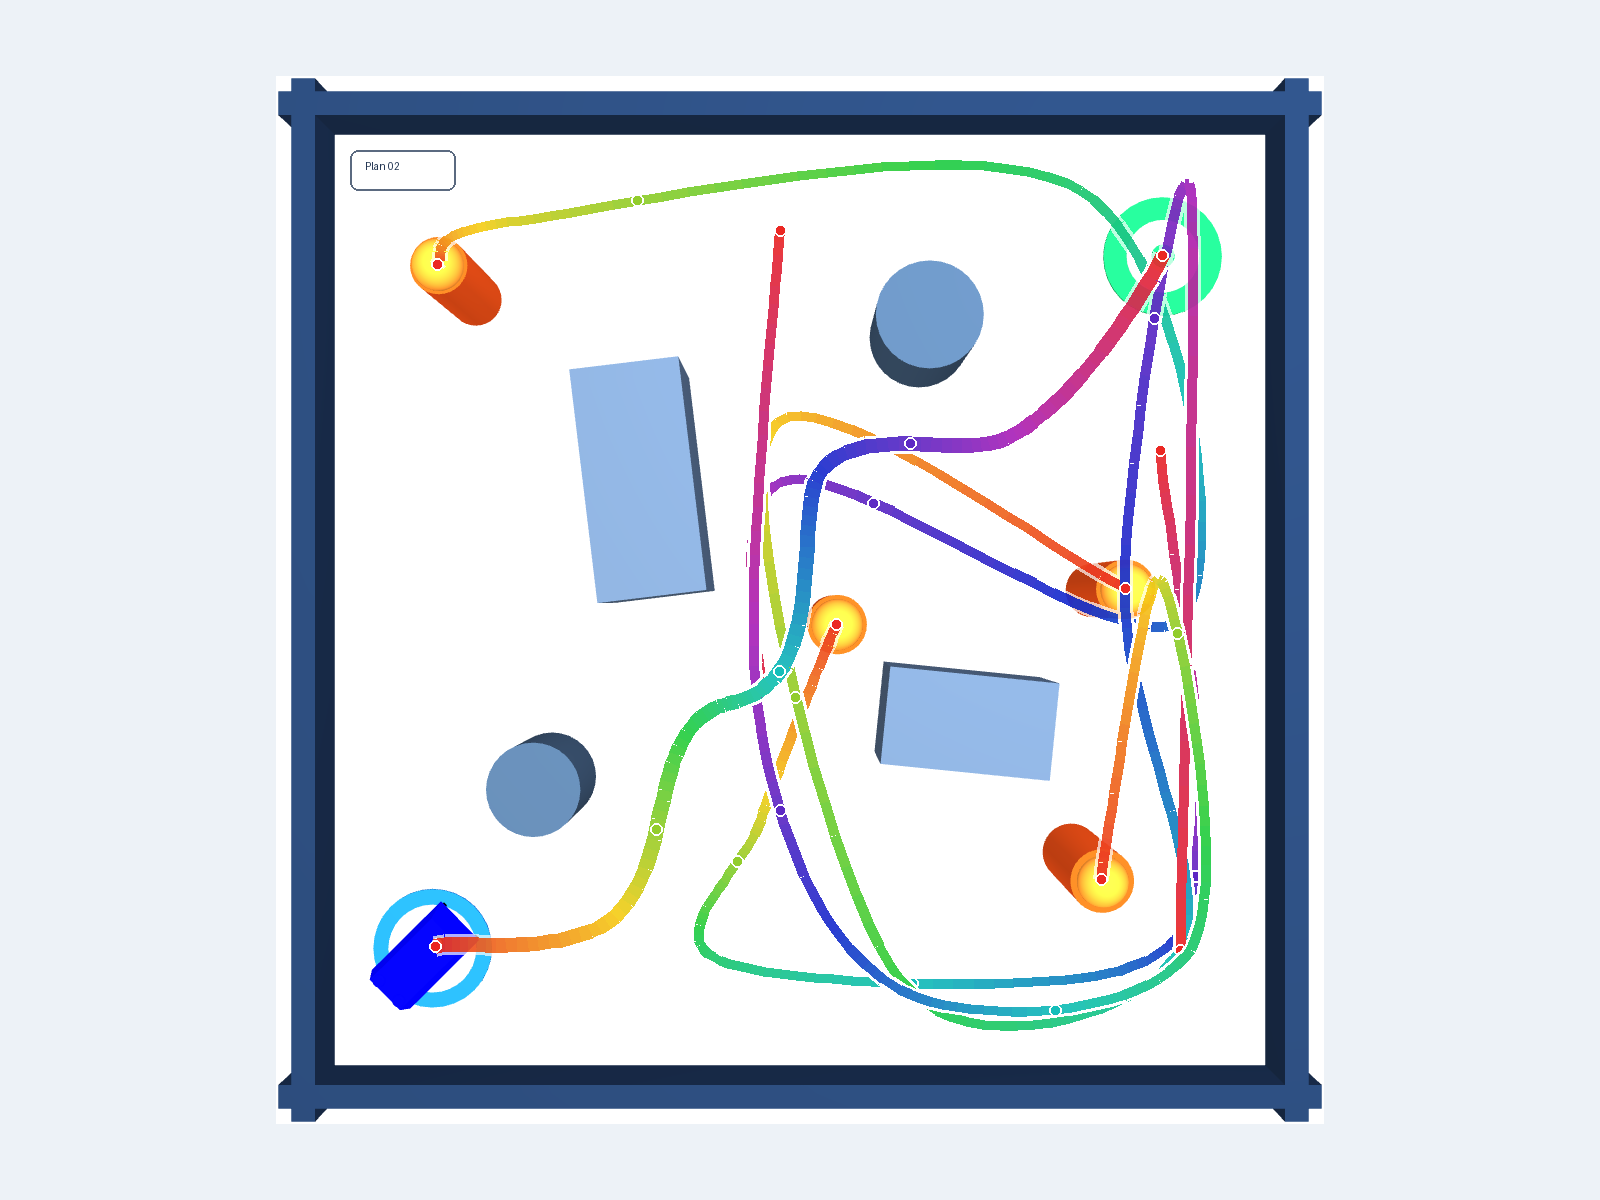
\includegraphics[width=\linewidth]{../rainbow_trajectory_synced_wavy_candidates_v3/rainbow_plan_02.png}
        \caption{密集轨迹交汇（Plan 02）}
    \end{subfigure}\hfill
    \begin{subfigure}[t]{0.32\textwidth}
        \centering

        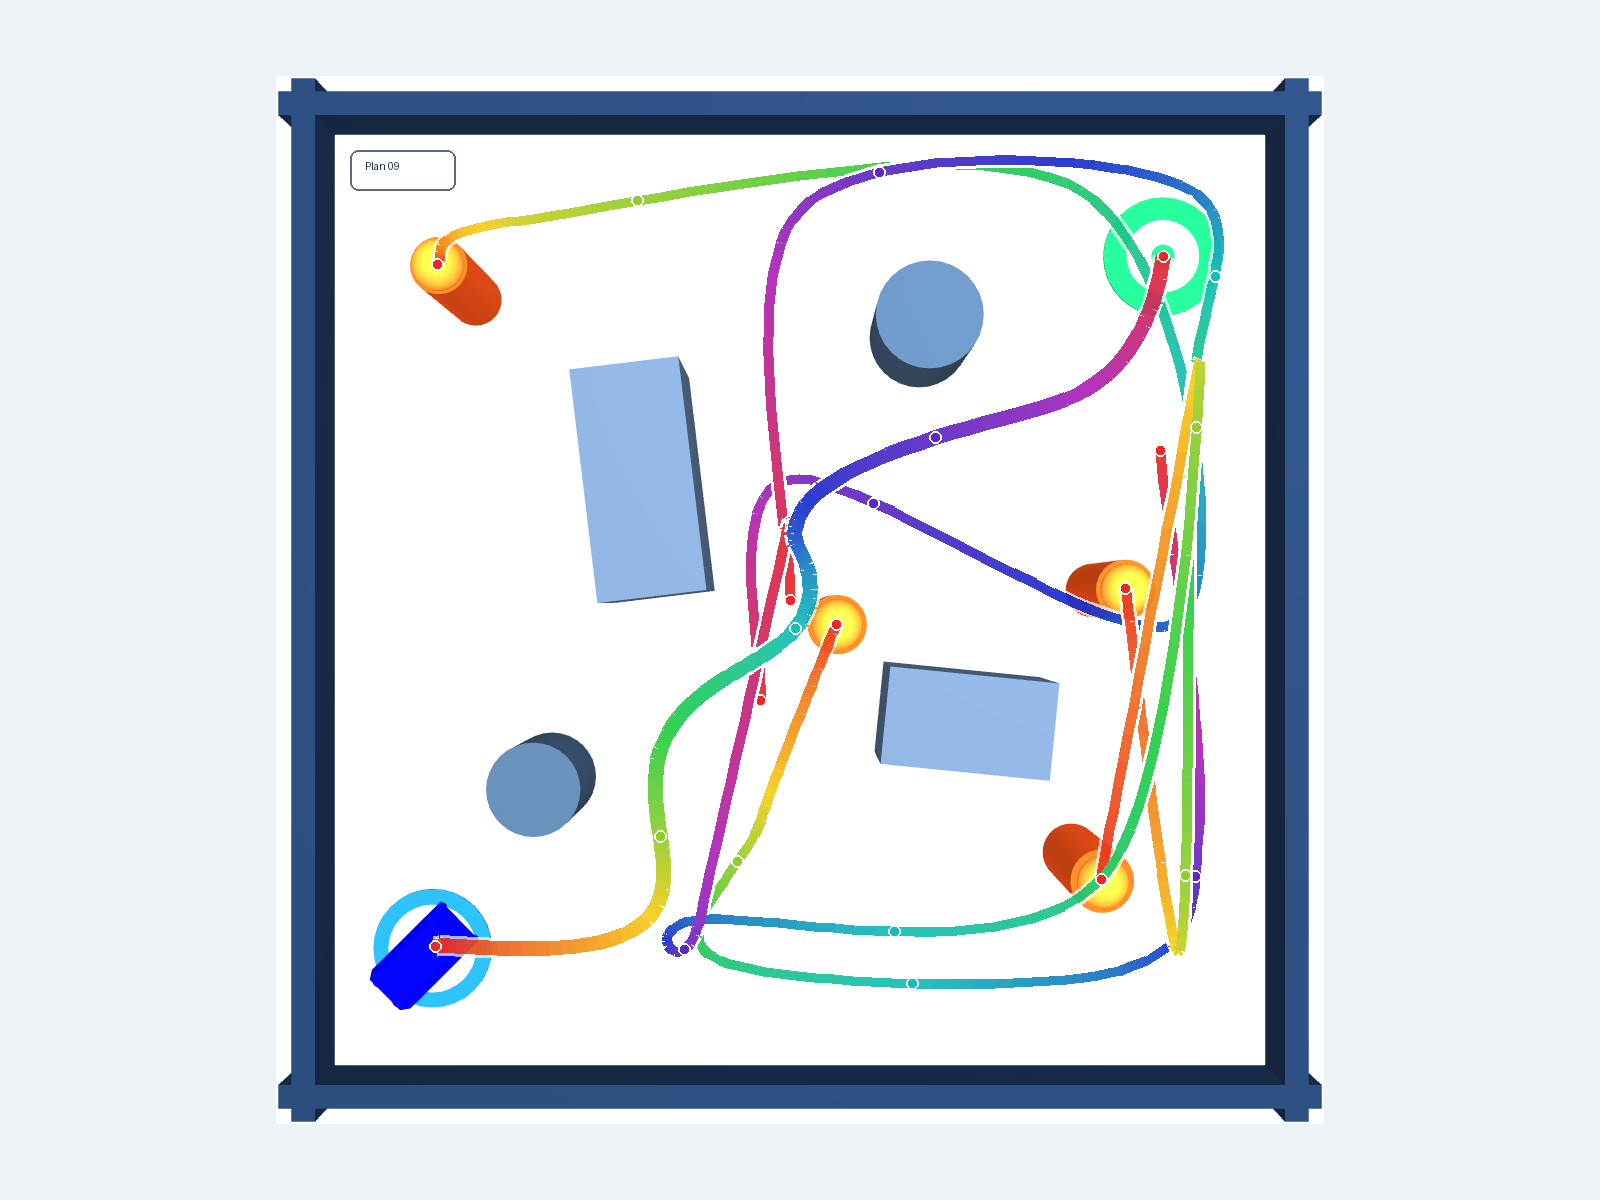
\includegraphics[width=\linewidth]{../rainbow_trajectory_synced_wavy_candidates_v3/rainbow_plan_09.png}
        \caption{边界绕行（Plan 09）}
    \end{subfigure}\hfill
    \begin{subfigure}[t]{0.32\textwidth}
        \centering

        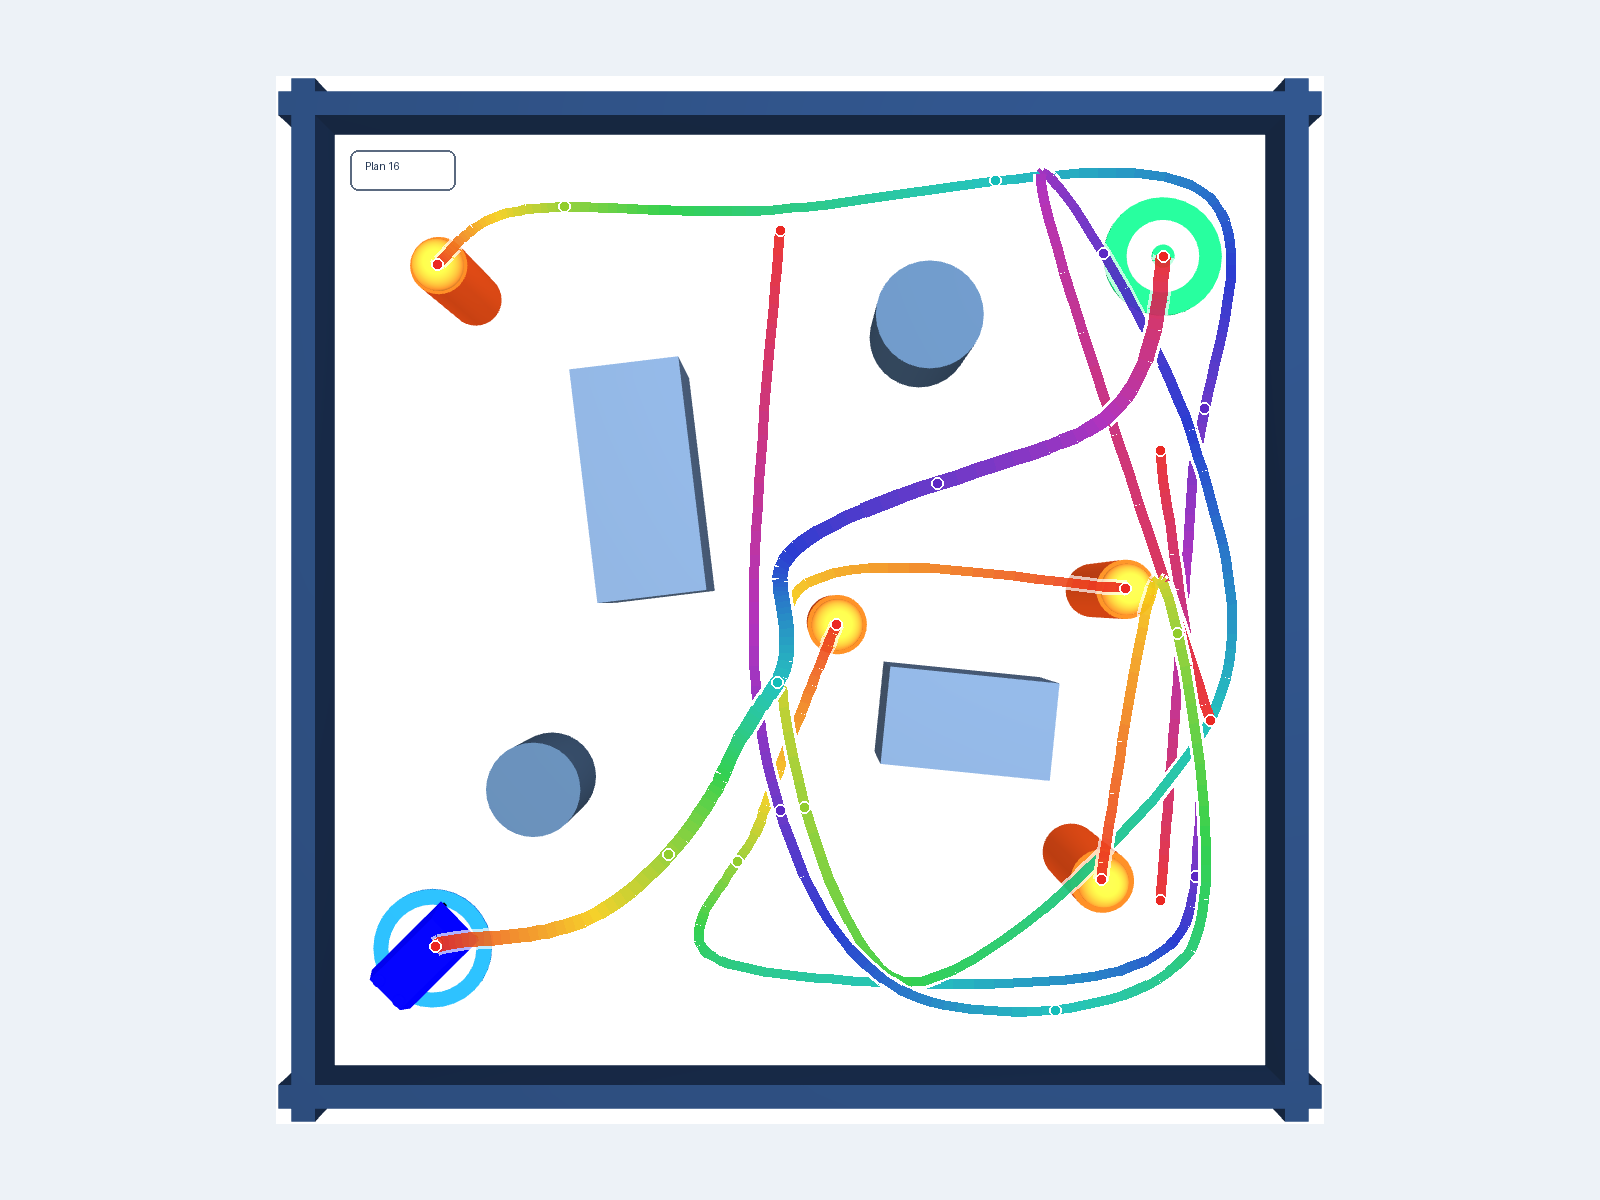
\includegraphics[width=\linewidth]{../rainbow_trajectory_synced_wavy_candidates_v3/rainbow_plan_16.png}
        \caption{多动态障碍交互（Plan 16）}
    \end{subfigure}
    \caption{Gazebo 动态场景中的时间同步彩虹轨迹。三幅图使用相同的场景布局，但对应不同的代表性运行样例。轨迹颜色编码仿真时间，相同颜色的采样点表示同一时刻；该同步表达可用于判断机器人与动态障碍物是否在空间交汇处发生时间重叠。}
    \label{fig:gazebo_rainbow_trajectories}
\end{figure*}

从三组轨迹可以看到，小车并未沿左下角至右上角的几何最短线直接穿越场景，而是在接近中部矩形障碍物、右侧运动柱体及目标邻域时主动改变曲率并保留空间间隔。尤其在多条轨迹发生几何交叉的位置，对应采样点通常具有不同颜色，说明机器人与障碍物通过错开到达时间避免了同时占据交汇区域。该现象从过程层面表明策略能够根据动态占用关系调整运动，而非仅对静态地图执行固定路径跟踪。该图只提供行为层面的定性证据，任务成功率、碰撞率与效率结论均以随后给出的 IRSim 多随机种子结果为依据。

\subsection{定量性能与消融}

表~\ref{tab:main_results} 和表~\ref{tab:efficiency_results} 汇总了 10 个随机种子、每种方法 200 个 episode 的结果。所有指标均以种子内均值为统计单元，报告跨种子的均值与标准误。图~\ref{fig:paper_rates} 对比任务终止类型。

\begin{table}[H]
    \centering

    \caption{不同导航策略的任务完成结果}
    \label{tab:main_results}
    \scriptsize

    \resizebox{\linewidth}{!}{\begin{tabular}{lccc}
\toprule
方法 & 成功率 $\uparrow$ & 碰撞率 $\downarrow$ & 超时率 $\downarrow$ \\
\midrule
DRL-VO & 60.0 $\pm$ 3.2 & 36.0 $\pm$ 4.0 & 4.0 $\pm$ 2.4 \\
PVO & 64.0 $\pm$ 5.1 & 30.0 $\pm$ 6.3 & 6.0 $\pm$ 4.0 \\
AVO & 76.0 $\pm$ 6.8 & 10.0 $\pm$ 6.3 & 14.0 $\pm$ 5.1 \\
AVO-UQ & 60.0 $\pm$ 7.1 & 4.0 $\pm$ 2.4 & 36.0 $\pm$ 6.8 \\
\bottomrule
\end{tabular}
}
\end{table}

\begin{figure}[H]
    \centering

    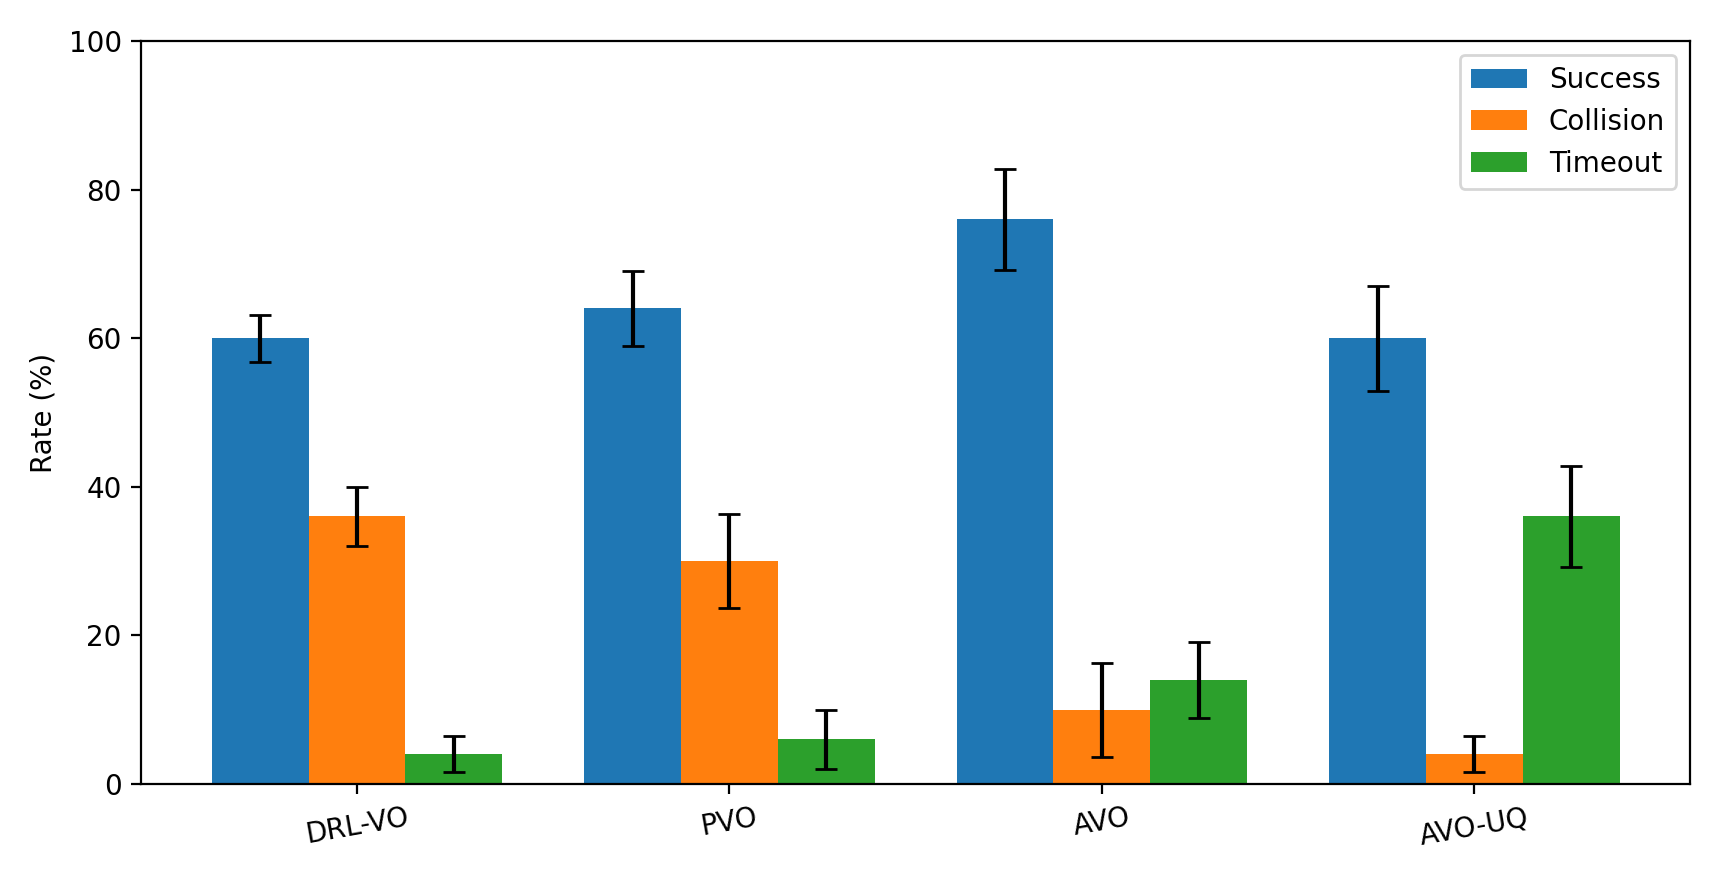
\includegraphics[width=0.95\linewidth]{../experiments/paper_results/paper_pvo_main_rates.png}
    \caption{多随机种子实验的成功率、碰撞率和超时率对比。误差线表示 per-seed 标准误。}
    \label{fig:paper_rates}
\end{figure}

\begin{table}[H]
    \centering

    \caption{不同导航策略的效率与模式指标}
    \label{tab:efficiency_results}
    \scriptsize

    \resizebox{\linewidth}{!}{\begin{tabular}{lccccc}
\toprule
方法 & 步数 $\downarrow$ & 路径 $\downarrow$ & 切换次数 $\downarrow$ & 侧/平比例 & 耗时/ms $\downarrow$ \\
\midrule
DRL-VO & 41.80 $\pm$ 8.12 & 2.67 $\pm$ 0.14 & -- & -- & 0.58 $\pm$ 0.03 \\
PVO & 8.03 $\pm$ 1.25 & 1.25 $\pm$ 0.18 & 0.91 $\pm$ 0.06 & 88.5 $\pm$ 6.1 & 6.31 $\pm$ 0.40 \\
AVO & 96.34 $\pm$ 12.45 & 4.20 $\pm$ 0.41 & 14.55 $\pm$ 1.85 & 48.6 $\pm$ 7.2 & 7.40 $\pm$ 0.10 \\
AVO-UQ & 108.57 $\pm$ 7.62 & 3.02 $\pm$ 0.48 & 17.67 $\pm$ 1.74 & 37.0 $\pm$ 5.2 & 5.63 $\pm$ 0.58 \\
\bottomrule
\end{tabular}
}
\end{table}

表~\ref{tab:efficiency_results} 中的“--”表示对应对比实现未记录逐时刻离散运动模式标签，因而不纳入模式切换与侧移/平移占比统计；该缺失项不表示方法采用了不同的机器人底盘。

首先，普通 PVO 的成功率为 $64.0\%\pm5.1\%$，略高于 DRL-VO 的 $60.0\%\pm3.2\%$；碰撞率则由 $36.0\%\pm4.0\%$ 降至 $30.0\%\pm6.3\%$。由于两者均运行在 4WIS 平台上，这一差异不再解释为底盘机动性变化，而反映当前帧碰撞判断从确定性 VO 扩展为概率危险集合后的有限收益。普通 PVO 能吸收一定的状态与速度估计误差，但仍受单帧恒速外推和零时延预测起点限制，因此碰撞率下降幅度有限。

进一步加入动作条件未来风险过滤后，AVO 的成功率提升至 $76.0\%\pm6.8\%$，碰撞率降至 $10.0\%\pm6.3\%$。相对于普通 PVO，成功率提高 12 个百分点、碰撞率降低 20 个百分点，但超时率也由 $6.0\%$ 增至 $14.0\%$。这组基准结果表明，在当前任务中，仅对当前帧速度障碍进行概率化的收益有限，而候选动作与短时未来占据的联合判断能够提供更有效的动作筛选。该结果反映的是动作条件风险模块在基础场景中的整体收益；历史长度、有效时延和运动模式的独立影响由表~\ref{tab:controlled_frequency}--表~\ref{tab:controlled_history} 的受控实验分别展开。AVO 的平均步数和路径长度分别增至 $96.34\pm12.45$ 和 $4.20\pm0.41$，说明硬安全筛选通过更长的绕行和等待换取碰撞下降。

AVO-UQ 将碰撞率进一步降至 $4.0\%\pm2.4\%$，但成功率回落至 $60.0\%\pm7.1\%$，超时率升至 $36.0\%\pm6.8\%$，平均步数达到 $108.57\pm7.62$。因此，不确定性惩罚并非无代价的安全增益：在缺少风险校准与停滞恢复机制时，额外保守性会把部分碰撞转化为超时。该消融揭示的不是单一“最优方法”，而是风险容忍度、任务完成率与通行效率之间可被明确调节的三方权衡。

\subsection{控制频率与有效反应窗口}

表~\ref{tab:controlled_frequency} 给出了固定观测频率 $50$ Hz 时的控制频率结果。控制频率从 $5$ Hz 提升到 $50$ Hz 后，AVO 的 $T_{\mathrm{eff}}$ 从 $245$ ms 降至 $65$ ms，成功率从 $58\%$ 提升至 $73\%$，碰撞率从 $22\%$ 降至 $13\%$；普通 PVO 的成功率从 $50\%$ 提升至 $69\%$，碰撞率从 $30\%$ 降至 $20\%$。这说明缩短动作更新间隔本身就能改善所有方法的反应能力，因此不宜把高频条件下的全部收益归因于历史建模。与此同时，在 $20$ Hz 和 $50$ Hz 条件下，AVO 的成功率分别为 $74\%$ 和 $73\%$，差异已经很小，呈现出高频端的边际收益减弱。

AVO-UQ 在相同频率扫描中始终保持更低碰撞率，$5$ Hz 时为 $10\%$，$50$ Hz 时为 $5\%$，但超时率分别为 $40\%$ 和 $29\%$。因此，UQ 分支主要扩大了安全裕度，而不一定提升任务完成率。表中单步推理耗时约为 $0.65$--$7.47$ ms，低于 $50$ Hz 控制周期的 $20$ ms；在该实验中，$T_{\mathrm{eff}}$ 的主要变化来自采样与控制更新间隔，而非推理模块本身。

\subsection{端到端时延鲁棒性}

表~\ref{tab:controlled_latency} 固定控制频率为 $20$ Hz，并逐步加入 $0$--$300$ ms 的附加时延。随着 $T_{\mathrm{eff}}$ 增大，所有方法的成功率下降、碰撞率上升，但动作条件未来风险的退化速度较慢。以 $300$ ms 为例，AVO 的成功率为 $55\%$、碰撞率为 $28\%$，相对于普通 PVO 的 $39\%$ 和 $43\%$ 分别高出 16 个百分点、低 15 个百分点。AVO-UQ 的碰撞率进一步降至 $18\%$，但超时率达到 $36\%$，再次体现保守筛选的效率代价。

时延还影响风险分数的可校准性。普通 PVO 的 Brier score/ECE 从 $0.11/0.07$ 增至 $0.21/0.14$，AVO 从 $0.08/0.040$ 增至 $0.14/0.080$，AVO-UQ 从 $0.060/0.030$ 增至 $0.100/0.070$。这一趋势表明，历史与动作条件风险并未消除时延造成的预测困难，但能够在更长有效反应窗口下保留相对稳定的排序能力；这正是将预测起点从当前时刻移向动作生效后的未来窗口的实验含义。

\subsection{障碍物运动模式边界}

表~\ref{tab:controlled_motion} 按障碍物未来运动复杂度排列了结果。在恒速运动下，普通 PVO、AVO 的成功率分别为 $74\%$ 和 $77\%$，碰撞率分别为 $15\%$ 和 $10\%$，两者差距较小，符合恒速假设较为匹配的条件。运动模式变为恒加速度、平滑转向、停止--启动和突然反向后，AVO 相对于普通 PVO 的成功率差值依次扩大为 $9$、$11$、$15$ 和 $17$ 个百分点，碰撞率差值扩大为 $11$、$11$、$13$ 和 $16$ 个百分点。该结果序列将方法收益与障碍物运动非线性联系起来，而不是笼统地宣称单帧 VO 在所有场景中失效。

局部遮挡条件进一步放大了状态不足的影响：普通 PVO 的成功率下降到 $40\%$、碰撞率上升到 $41\%$，而 AVO 仍达到 $58\%$ 成功率和 $24\%$ 碰撞率。AVO-UQ 在六种模式下均取得最低碰撞率，但超时率处于 $31\%$--$40\%$，说明其更适合作为安全优先配置，而不应仅以成功率作为评价依据。

\subsection{历史状态与状态质量消融}

表~\ref{tab:controlled_history} 进一步把历史长度、有效时延和状态来源放在同一组条件中比较。当前帧条件下，AVO 的成功率为 $68\%$、碰撞率为 $20\%$，与单帧 PVO 的 $67\%$ 和 $21\%$ 接近；将历史窗口从 $K=1$ 增加到 $K=3$ 和 $K=5$ 后，AVO 的成功率分别提升到 $72\%$ 和 $75\%$，碰撞率下降到 $15\%$ 和 $11\%$。与此同时，AUROC 从 $0.70$ 提升到 $0.77$ 和 $0.83$，ECE 从 $0.08$ 降至 $0.07$ 和 $0.05$，同时体现出风险排序能力和概率校准能力的改善。

加入 $50$ ms 附加时延后，$K=5$ 的成功率回落到 $70\%$，碰撞率升至 $15\%$，说明历史信息提供了补偿但不足以完全抵消更长的有效反应窗口。Oracle state reference 下，$K=5$ 的 AVO 达到 $78\%$ 成功率、$9\%$ 碰撞率、$0.90$ AUROC 和 $0.03$ ECE；相对于估计状态的 $K=5$ 条件仍有差距，表明感知状态质量是影响风险预测的关键因素。表 9 的 AUROC/ECE 用于量化历史风险头的判别能力和概率校准能力；DRL-VO 不输出概率，因此相关校准指标记为 N/A。

\section{讨论}

上述结果形成了由“基准收益”到“适用边界”的两层证据链。在相同 4WIS 平台上，普通 PVO 相比 DRL-VO 仅获得有限改善，而 AVO 相比普通 PVO 同时降低碰撞率并提高成功率，说明候选动作条件和短时未来占据推演比单纯概率化当前帧风险更有效。控制频率实验进一步表明，高频滚动更新本身就能改善所有方法的反应能力；时延和运动模式实验则显示，当有效反应窗口变长或障碍物运动偏离恒速时，AVO 的相对优势更加明显。由此，本文的核心论点应表述为条件性命题：历史和未来风险建模的价值取决于状态是否覆盖动作生效前后的关键时间段。

AVO-UQ 的结果揭示了另一项重要权衡。它在频率扫描、时延扫描和运动模式扫描中通常取得最低碰撞率，但超时率持续偏高，说明保守风险修正把部分碰撞风险转化为等待、绕行和任务超时。因此，实际系统不应只优化碰撞率，而应联合考虑成功率、碰撞率、超时率、最小安全距离、路径长度和干预频率，并根据应用场景选择风险阈值。

表 6--表 9 汇报实际受控实验结果，其中表 9 的 AUROC 和 ECE 来自历史风险头的状态消融与概率校准流程。各受控条件均采用 $N=200$ 个 episode，表中给出条件级点估计，并与基准实验的跨种子统计共同刻画方法的安全性、效率和适用边界。

此外，4WIS 定量仿真采用理想化平面运动学，未显式建模轮级转角约束、转向速率上限和执行器动态；Gazebo 轨迹主要承担过程级行为展示。因此，本文结论主要针对统一 4WIS 运动学平台、给定感知条件和所报告有效反应窗口成立。

\section{结论}

本文将问题限定为：在部分可观测且有效反应窗口不可忽略时，当前状态是否足以支持 4WIS 多模态候选动作的安全判断。为此，AVO 将碰撞风险表示为观测历史、候选动作和未来执行窗口的联合函数，并将风险评估嵌入动作执行前的安全过滤。四种方法均在同一 4WIS 平台上比较；基础多随机种子结果中，AVO 相对于普通 PVO 将成功率从 $64.0\%\pm5.1\%$ 提升至 $76.0\%\pm6.8\%$，将碰撞率从 $30.0\%\pm6.3\%$ 降至 $10.0\%\pm6.3\%$；AVO-UQ 将碰撞率进一步降至 $4.0\%\pm2.4\%$，代价是超时率升至 $36.0\%\pm6.8\%$。

表 6--表 9 的受控实验把这一结论展开为四个可检验维度：控制频率决定有效反应窗口的长度，端到端时延决定当前观测与动作生效之间的错位，障碍物运动模式决定恒速外推的适用程度，历史窗口和状态来源决定风险预测所能恢复的动态信息。结果呈现出清晰的边界趋势：高频、低时延和恒速条件下各方法差距缩小；时延增加、运动转向或局部遮挡出现后，动作条件未来风险的优势扩大；不确定性修正则以更高超时为代价换取更低碰撞率。


\bibliographystyle{ieeetr}
\bibliography{references}

\end{document}
